\documentclass[11pt,a4paper]{report}

% Aberstwyth MMP Project Report Template for LaTeX
%
% Authors: Neil Taylor (nst@aber.ac.uk) and Dr. Hannah Dee (hmd1@aber.ac.uk) 
%
% This has been adapted from the Leeds Thesis template and the 
% Group Project template for Computer Science in Aberystywth University.
% 
% All comments and suggestions welcome.
%
% Template designed to be used with pdflatex: it may need alteration to
% run with a different LaTeX engine.
%
% Note - this is offered as a starting point for your work. You are not 
% required to use this template and can choose to create your own document 
% without it.

% This template is suitable for students with an engineering-style project, 
% which will be most students in the department. If your project is a research-oriented 
% project, look at the alternative template.

% To build document on the unix command line, run four commands:
 
% pdflatex mmp-report
% bibtex mmp-report
% pdflatex mmp-report
% pdflatex mmp-report

\usepackage{pdfpages}

% you will end up with mmp-report.pdf. Before submitting, add your user ID as a prefix, 
% e.g. abc01-mmp-report.pdf 
\usepackage{StylesAndReferences/mmp-report}

% the following packages are used for citations - You only need to include one. 
%
% Use the cite package if you are using the numeric style (e.g. IEEEannot). 
% Use the natbib package if you are using the author-date style (e.g. authordate2annot). 
% Only use one of these and comment out or remove the other one. 
\usepackage{cite}
%\usepackage{natbib}

%%%% Title and Section Colours %%%%
% Modify these values to change the colours used for title, sections and subsections.
% Each value is a range of 0-255 in RGB colourspace.
% Idea courtesy of discussion at 
% https://www.overleaf.com/learn/latex/Using_colours_in_LaTeX
% and
% https://tex.stackexchange.com/questions/75667/change-colour-on-chapter-section-headings-lyx
% 
% If you prefer to have black headers, then comment out the following lines
\definecolor{mmpTitle}{RGB}{0, 0, 0}
%\definecolor{mmpSection}{RGB}{10,85,155}
%\definecolor{mmpSubsection}{RGB}{79,129,189}

%\chapterfont{\color{mmpTitle}}  % sets colour of chapters
%\sectionfont{\color{mmpSection}}  % sets colour of sections 
%\subsectionfont{\color{mmpSubsection}} % sets colour subsections
%\subsubsectionfont{\color{mmpSubsection}} % sets colour subsections

%%%% end of Title and Section Colours %%%%


%%%% Report Type %%%%
%% comment/uncomment depending on the type of report you want to generate
\reporttype{Engineering}
%\reporttype{Research}
%%%% end of Report Type %%%%


\begin{document}

%TC:ignore

% all of the include directives below refer to tex files
% so %TC:ignore 

\title{Tax-E - Android App for Local Taxi Bookings}

% Your name
\author{Rhys Evans}

% Your email 
\authoremail{rhe24@aber.ac.uk}

\degreeschemecode{G400} %e.g. G400 
\degreeschemetitle{Computer Science} % e.g. Computer Science
\degreetype{BSc}

\modulecode{CS39440} % i.e. CS39440, CC39440, CS39620
\moduletitle{Major Project} % i.e. Major Project or Minor Project

\date{3rd May 2019} % i.e. the date of the current version of your report

\status{Release} % Use draft until you create the release version. Then, change this to Release.
\version{1.0}

% The title and name of your supervisor.
\supervisor{Chris Loftus} 

%The email for your supervisor. 
\supervisoremail{cwl@aber.ac.uk}

\maketitle

%TC:endignore
 includes cover.tex - to change the content,
% edit the tex file

\pagenumbering{roman}

% This is the front page
%TC:ignore 

\title{Tax-E - Android App for Local Taxi Bookings}

% Your name
\author{Rhys Evans}

% Your email 
\authoremail{rhe24@aber.ac.uk}

\degreeschemecode{G400} %e.g. G400 
\degreeschemetitle{Computer Science} % e.g. Computer Science
\degreetype{BSc}

\modulecode{CS39440} % i.e. CS39440, CC39440, CS39620
\moduletitle{Major Project} % i.e. Major Project or Minor Project

\date{3rd May 2019} % i.e. the date of the current version of your report

\status{Release} % Use draft until you create the release version. Then, change this to Release.
\version{1.0}

% The title and name of your supervisor.
\supervisor{Chris Loftus} 

%The email for your supervisor. 
\supervisoremail{cwl@aber.ac.uk}

\maketitle

%TC:endignore
                        

% Set up page numbering
\pagestyle{empty}

% declarations of originality 
\thispagestyle{empty}

%TC:ignore

%%%
%%% You must sign the declaration of originality. 
%%%
%%% You are submitting this electronically. Therefore, to sign, you 
%%% type your name and date to replace the .... characters. 
%%%
\section*{\centering Declaration of originality}

I confirm that:

\begin{itemize}
\item{This submission is my own work, except where 
clearly indicated.}

\item{I understand that there are severe penalties for Unacceptable Academic Practice, which can lead to loss of marks or even the withholding of a degree.}
 
\item{I have read the regulations on Unacceptable Academic Practice from the University's Academic Registry (AR) and the relevant sections of the current Student Handbook of the Department of Computer Science.}
 
\item{In submitting this work I understand and agree to abide by the University's regulations governing these issues.}
\end{itemize}

\vspace{2em}
Name: Rhys Evans \\

\vspace{1em}
Date: 23rd April 2019 \\

%%% 
%%% We would like to make a selection of final reports available to students that take 
%%% this module in future years. To enable us to do this, we require your consent. You 
%%% are not required that you do this, but if you do give your consent, then we will have 
%%% the option to select yours as one of a number of reports as examples for other 
%%% students. If you would like to give your consent, then please include the following 
%%% text and type your name and date to replace the .... characters. 
%%% 
%%% If you do not wish to give your consent, please remove this from your report. 
%%%
\vspace{1em}
\section*{\centering Consent to share this work}

By including my name below, I hereby agree to this project's report and technical work being made available to other students and academic staff of the Aberystwyth Computer Science Department.  

\vspace{2em}
Name: Rhys Evans \\

\vspace{1em}
Date: 23rd April 2019 \\

%TC:endignore

               

\thispagestyle{empty}

%TC:ignore

\section*{\centering Acknowledgements}

I would like to thank the following people for their invaluable support and guidance throughout this project: \\

My project supervisor, Chris Loftus for allowing me to pursue this project and going above and beyond to support me throughout. His organization of the weekly progress meetings was thoroughly helpful, allowing me to reflect on my progress and receive genuine feedback on various aspects of implementation. \\

My caring partner, Sara for providing me with continuous support, motivation and inspiration. Her honest and constructive feedback on the app's development was invaluable. \\

My loving family, John, Davina, Carwyn and Delyth for always being there and believing in me.


%TC:endignore % Acknowledgements

\thispagestyle{empty}

%TC:ignore

\section*{\centering Abstract}

Web and Mobile Technologies have become increasingly ubiquitous in the travel and tourism industry. These technologies, together with a company's ability to successfully adopt them is often pivotal to the company's success within the industry.

This project's aim was to provide a platform for local taxi companies to interact with and provide a service for their customers. The key aspect of the platform is the creation, viewing, and management of bookings. By handling bookings this way, customers and taxi companies can reliably keep track of their past and present bookings in real time.

This project has produced a fit for purpose, fully functional platform. It is split into 3 key systems: a REST API to interact with the backend database and be consumed by other systems within the platform; a web app to be used by controllers within a company to claim, delegate, and manage bookings; and an Android App to be used by customers and drivers to view, create, and manage bookings. The developed product is flexible, allowing taxi companies to choose the level of adaptation that would best fit their business.

Predictably, however, there is room for improvement and future development within the project. Given the scope and time restrictions provided, the produced platform is only intended as a starting point and proof of concept.

This document will provide an insight into the motivation behind platform's development, address weaknesses and key areas for improvement, and discuss the engineering and project management challenges encountered and how they were overcome.

%TC:endignore                 % Abstract

\pagenumbering{roman}
\pagestyle{fancy}
\fancyhead{}
\fancyfoot[C]{\thepage}
\renewcommand{\headrulewidth}{0 pt}
\renewcommand{\chaptermark}[1]{\markboth{#1}{}}

\tableofcontents   
\newpage
\listoffigures % comment out this line if you don't have any figures / graphics
\newpage 
%\listoftables % comment out this line if you don't have any tables
\newpage

% Set up page numbering
\pagenumbering{arabic}

\setchapterheaderfooter

%TC:endignore

% include the chapters
\chapter{Background \& Objectives}

This section should discuss your preparation for the project, including background reading, your analysis of the problem and the process or method you have followed to help structure your work.  It is likely that you will reuse part of your outline project specification, but as you write this report at the end of the project you should have more to discuss. 

\textbf{Note}: 

\begin{itemize}
   \item All of the sections and text in this example are for illustration purposes. The main Chapters are a good starting point, but the content and actual sections that you include are likely to be different.
   
   \item Look at the document MMP\_SO8 Project Report and Technical Work \cite{ProjectReportTechicalWork} for additional guidance. 
   
\end {itemize}

\section{Background}
What was your background preparation for the project? What similar systems did you assess? What was your motivation and interest in this project?

\section{Analysis}
Taking into account the problem and what you learned from the background work, what was your analysis of the problem? How did your analysis help to decompose the problem into the main tasks that you would undertake? Were there alternative approaches? Why did you choose one approach compared to the alternatives? 

There should be a clear statement of the objectives of the work, which you will evaluate at the end of the work. 

In most cases, the agreed objectives or requirements will be the result of a compromise between what would ideally have been produced and what was determined to be possible in the time available. A discussion of the process of arriving at the final list is usually appropriate.

As mentioned in the lectures, think about possible security issues for the project topic. Whilst these might not be relevant for all projects, do consider if there are relevant for your project. Where there are relevant security issues, discuss how they will this affect the work that you are doing. Carry forward this discussion into relevant areas for design, implementation and testing.

\section{Process}
You need to describe briefly the life cycle model or research method that you used. You do not need to write about all of the different process models that you are aware of. Focus on the process model that you have used. It is possible that you needed to adapt an existing process model to suit your project; clearly identify what you used and how you adapted it for your needs.


%\addcontentsline{toc}{chapter}{Development Process}
\chapter{Design}
This chapter will discuss the overall architecture and higher level aspects of the platform's design. It is only intended to provide an overview of the design. A more in-depth discussion of specific design decisions will be presented on a per-iteration basis later in the report.

\section{Overall Architecture}
The platform is comprised of 3 key systems: a REST API that interfaces with a MongoDB database; an Android App to consume the API and serve content to Customers and Drivers; a Responsive Web App to consume the API and serve content to Company Admins.

[INSERT OVERALL GRAPHIC / USE-CASE DIAGRAM?]

Both the Android and Web App are categorized as user-facing systems. Meaning the platform's users are never intended to interact with the API directly, but rather through one of these two Applications (depending on their role). This also means that the two user-facing  Applications never interact with each other, they exclusively send and receive data from the API. This is depicted in the sequence diagram below:

[INSERT SEQUENCE DIAGRAM]

Data received from the API is in JSON format, which is natively deserialized by Javascript and Typescript. However, Android's GSON library is used to support JSON conversion to and from 'plain old Java objects' (POJOs).

\section{REST API Architecture Overview}
Broadly, the REST API is a modular system split up into the following: models, services, controllers, routes, middlewares, and helpers.

The model module contains all the models for the system. These directly map onto a collection within the MongoDB database. Some models may reference each other using MongoDB ObjectIDs, comparable to SQL's foreign key constraint. Any model file can be referenced from anywhere within the system and used as a 'type' to initialize objects.

The services module is the lowest level of abstraction for interfacing with the backend database. It exposes several necessary public functions to the rest of the system. Typically, it will implement CRUD functions via mongoose. The service files are only intended to be accessible from their respective controllers.

Controllers are the next level up from services in the API's abstraction layers. Controller files are called by the API's router to pass information from the HTTP request to the required service. Then execute the relevant middleware. The functions within a controller file are typically very simple and simply serve as an intermediary between the router and the services themselves.

Routes are used to capture information from the HTTP request and pass it to the controllers so the relevant operations can be completed (via the service).  These include retrieving values from request headers, the request body, and any URL parameters or queries.

Several middleware files were created for the API, middleware is executed by the router before any code from the controller is executed. Middleware can be configured to run on every route or to be executed on a per-route basis. For example, the error handling middleware needs to be executed on every route. However, a piece of middleware such as access control or authentication may only need to be executed on certain protected routes.

[INSERT DIAGRAM TO SHOW ORDER OF EXECUTION OF MIDDLEWARE]

Helpers do not have a designated place in the order of execution of requests. Rather, they are intended to be used by other modules within the API to perform frequent, utility tasks or to enumerate types. For example, there are two enumeration types within the helper module 'role' and 'status'. These are used across many different modules within the API to reduce code duplication.

[INSERT DIAGRAM TO DEPICT THE ABSTRACTION LAYERS]

\section{Data Model}
The data model for the platform is fairly straight forward, the simple, flexible nature of MongoDB certainly assisted in this simplicity. To preface, a 'collection' in this context is comparable to a 'relation' in a traditional relational DBMS. A 'document' is comparable to a 'tuple' or 'record', and a 'field' is comparable to a 'column' or 'attribute'.

The data model contains three collections 'User', 'Booking', and 'Company'. All collections have unique Object IDs and each collection references another. The 'User' collection is likely the largest, it is a general model for Customers, Drivers, and Company Admins. The decision to use a single, larger model for all users, as opposed to a specific model for each type of user was made early on, due to its simplicity. This is implemented by leaving the type-specific fields as null if they are not applicable to the user. A user's type is stored using the 'role' field. The data model is depicted in the Entity Relationship below:

[INSERT E-R DIAGRAM]

\section{Android App Architecture Overview}
Much of the Android App's design is boilerplate, with the main package split into java code and app resources. There are no significant differences between the app's build variants as it is intended to offer different functionality dynamically, depending on the user's role. It was considered early on to provide two different variants of the app, one for customers and another for drivers. However, as the differences between the two app's functionalities would be very minor it was decided that a single app would be the best approach.

The app's main java package is comprised of 5 packages: model, network, ui, util, and viewmodel.

[INSERT IMAGE OF ALL PACKAGES AND CLASSES]

The model package contains 5 model classes, each representing a type of JSON response that can be received from the API. They are required to enable serialization/de-serialization of JSON objects. The 'User', 'Booking', and 'Company', and 'Response' models are the ones uses most frequently. With 'LoginResponse' only being used in a single special case. The Response model is returned anytime the API is expected to return a generic response with no particularly important data. It is very useful for Error Handling for retrieval of JSON values.

The network package contains the classes required to interface with the API using Retrofit. It contains the 'RetrofitInterface' interface, which is comparable to the Repository interface that would be used in Android's data persistence library. The 'NetworkUtil' class has several overloaded methods that each return a differing instance of the RetrofitInterface. For example, if the method is called with no parameters it returns a Retrofit instance with no HTTP authentication headers. Whereas, if the method is called with an access token as a parameter, it returns a Retrofit instance with the access token in the HTTP headers.

All of the app's activity and fragment classes are located in the ui package. The package itself is split into 5 sub-packages, which are intended to relate to each of the app's screens and dialogs. The app has two main activities Authentication and Main. This is how access control is enforced in the app, the user can only access the main activity if they have successfully logged in via the authentication activity. There are of course other activities within the app, but they are always called on top of one of the two main activities.

The util package contains all of the classes that contain shared code that is intended to be used all across the app. This includes the app's error handler, validator, shared preference manager, customer de-serializers, enum types, and more. The use of a util package with these classes is intended to reduce code duplication.

The Model View ViewModel (MVVM) design pattern is implemented in this app via the viewmodel package. The view models within this package provide a layer of abstraction between the networking and UI classes. In the case that the API's routes were updated, supporting this update in the app is made considerably easier using view models. Therefore increasing maintainability and encouraging good object orientation practices.

[INSERT MVVM DIAGRAM]

\section{Web App Architecture Overview}
The Web Application is likely the simplest system within the platform. Similarly to the Android Application, the main directories are fairly similar to a boilerplate Angular Application. The main directory of the app contains seven sub-directories: '\_guards', '\_helpers', '\_models', '\_services', 'components', 'layouts', 'modules'.

The '\_guards' directory currently contains a single guard file to enforce authentication within the app.

The '\_helpers' directory contains two HTTP interceptors, an error interceptor, and an access token interceptor. The error interceptor is intended to intercept incoming responses from the API and handle any errors appropriately. If the application was of a larger scale, it would likely be more appropriate to also have a designated error handling file. However, due to the scale of the application currently, this solution was selected due to its simplicity. The 'jwt' interceptor is intended to intercept outgoing requests to the API and append the user's access token to the request headers. This means that the token doesn't have to be manually added each time a request is made.

The '\_services' directory contains all of the services required by various views. The services are intended to add a layer of abstraction between the view and the HTTP requests. There is also a service file for displaying notifications in the view, it works by injecting a HTML element into the view and running jQuery code to animate the element.

All of the app's angular components reside in the 'components' directory. An angular component represents a 'page' within the app, with components belonging to a module. For example, the 'drivers' page is a component that belongs to the 'main' module. Each component contains a view file, style file, and controller file. These are typically html, scsss, and typescript files respectively.

Any recurring layouts within the app reside in the 'layouts' directory. This includes things such as headers, footers, navbars, etc. Similarly to components, each layout has a view, style, and controller file. However, the layout directory is treated as its own Angular module.

Lastly, the modules directory contains the app's two main modules 'auth' and 'main', these modules create a scope in which components can exist. Each module requires a router and module file, in addition to the files required by standard components. A module's view file will typically contain a placeholder for whichever component the module's router serves.

[INSERT IMAGE DEPICTING ANGULAR APPLICATION LAYOUT]

\section{User Interface}

\section{Technologies Used}
As the developed platform would contain several systems, it was clear that a diverse array of technologies would need to be adopted. Both to aid project management and for use in implementation. This section will discuss the selected technologies for this project.

\subsection{Implementation}
With regards to the technology that would be used to develop the REST API, it was a close decision between Rails 5 and Node.js / Express.js. Although Flask and ASP.net were most certainly fit for purpose and had plenty of documentation to get started. There was a distinct lack of experience in the underlying languages (Python \& C\#). The project supervisor had a level of expertise in Rails, this would have been an advantage for the adoption of this framework. However, due to personal preference and a slight bias towards Javascript, Node.js together with Express.js was selected. This choice showed great promise, with a considerable amount of online resources and available testing libraries. It would also mean the development of the API would integrate seamlessly with Node.js's default package manager (NPM). This would allow access to hundreds of thousands of javascript packages.

Having researched both Angular and React it was clear they were both equally appropriate for this task. However, Angular's traits were increasingly more appealing after in-depth research. It offered a substantial amount of in-built functionality compared to React. Examples of these functionalities are an In-built XSS protection, a native Router (eliminating the need for a third party library), a form builder, and SCSS compiling. It also supported Google's Material Design, through pre-built components, this was ideal to ensure consistency between the platform's applications. The only considerable drawback was that Angular is based in Typescript, a syntactically strict superset of Javascript; this was an unfamiliar technology. However, given the considerable advantages and previous experience with Javascript, the benefits certainly outweighed the drawbacks. It should also be mentioned that the adoption of Angular would loosely complete the project's adoption of the MEAN stack~\cite{mean_documentation_ref}.

\subsection{Data Persistence}
Although the research was certainly a key part of making a fully informed decision; a JSON-like document-oriented DBMS seemed like an obvious fit, having already decided to use Node.js for the API. Therefore, MongoDB was selected.  One disadvantage of a NoSQL solution is that complicated queries are typically considered more difficult compared to a traditional SQL DBMS. However, given the simple nature of the queries for this project, this didn't seem overly relevant. 

\subsection{Development Environments}
Having researched JetBrains' WebStorm, it was decided it would be a better fit for the development of both the platform's REST API and Web Application. With substantial language-specific support, code completion, syntax highlighting, and a preview of markdown files, it was an easy decision. WebStorm also provides in-built integration with docker, GitHub, and NPM.

\subsection{Project Management}
After researching many project management solutions, a decision was made to use Docker for containerization of the REST API. This conclusion was mainly motivated by the ability to easily replicate the development environment across multiple machines. Due to Extreme Programming being the project's chosen development methodology, a Continuous Integration tool had to be selected. Having researched several options, it was eventually decided that TravisCI would be used. It was by far the most lightweight and easy to understand tool of those researched. It seamlessly integrates with GitHub through the use of a single YAML file and OAuth, making adoption relatively easy for inexperienced users.

\subsection{Deployment}
In order to make an informed decision regarding the deployment method for the API and Web Application, sample applications were deployed using both Heroku and AWS. It was discovered that the process was actually a lot more in-depth than initially anticipated. Together with having to register an account and provide banking details this was somewhat discouraging. Therefore the API and Web Application were both deployed to a home-based headless ubuntu-server box. The API is deployed using Nginx as a reverse proxy and Node.js's process manager, PM2. The Web Application is deployed using an Apache web server.

Although there are certain security implications with a 'homemade' deployment solution.  For example, the lack of reliable SSL encryption and physical security concerns due to the location of the server itself. The deployment is only intended for demonstration purposes and will likely only contain fictitious test data. If the platform were ever to be deployed for production, a fully supported commercial solution would be sought out.






\chapter{Implementation}
The implementation phase of this project spanned across 9 weeks. Given that the software development methodology adopted was Extreme Programming. The platform was implemented with an iterative approach or a series of 'Weekly Cycles'. In this chapter, an overview of the work done in each weekly cycle will be provided, including a discussion of any problems encountered and how they were overcome.

As discussed in Section~\ref{process_ref}, at the beginning of each week it was decided which stories would be completed, with some non-essential stories included to add slack.

\begin{figure}[!htb]
	\centering
	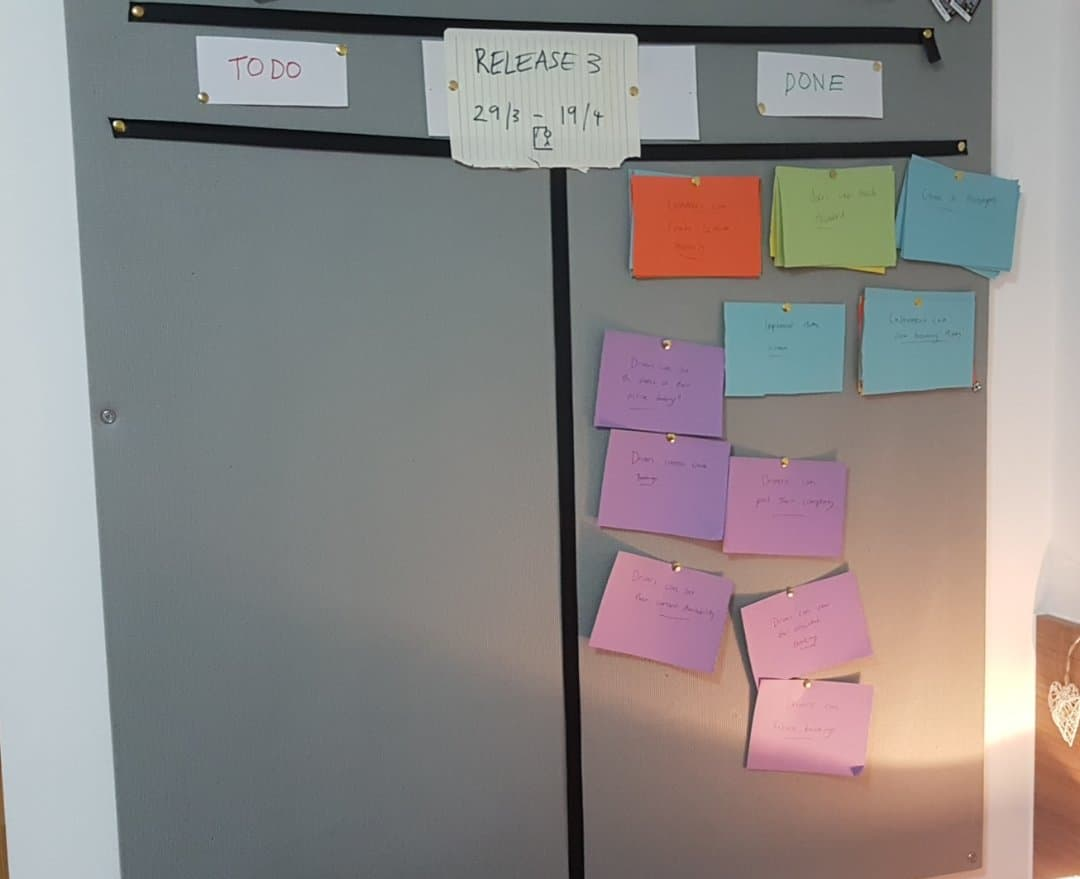
\includegraphics[width=0.5\linewidth]{Resources/img/story_board.jpg}
	\caption{The physical Story Board used throughout the project}
	\label{fig:story-board}
\end{figure}

\section{Week 1 (15/02 - 22/02)}
All the required prototyping for the platform took place in the first week of development. This included UI Prototypes for the Android App's screens, a prototype Authentication API, and a prototype Android App to consume the Authentication API.

\subsection{Prototype Authentication API}
During the creation of the prototype Authentication API, research into third-party authentication libraries was also done, with libraries such as Okta~\cite{okta_documentation_ref} and Passport.js~\cite{passport_documentation_ref} being considered. It was eventually decided, however, that a custom solution would allow for more fine-grain control over the API's authentication and access control.

\subsection{Prototype Android App}
Using the created API, the next task was to create a prototype Android App to consume the API. A major part of this task was to set up HTTP requests and JSON response de-serialization. The second tutorial in Raj Amal's series of walkthroughs~\cite{nodejs_authentication_tutorial_ref} proved essential in understanding Retrofit, rxJava, and Google's GSON. The prototype App allowed users to register, login, and view their profile. It enforced access control to ensure un-authenticated users couldn't view the main screen of the App. The Android aspect of this implementation was fairly trivial due to previous experience. For example, storing the user's access token in shared preferences and limiting access by requiring the presence of the token.

\subsection{User Interface Prototypes}
Now that there were prototypes in place to lay the foundation, it was time to prototype the User Interface for the actual platform. The first step in this process was to establish a general style and branding. This involved deciding on a colour scheme, choosing a typeface, and creating the first draft of the platform's logo. The remainder of the work involved actually creating the prototype for each of the App's screen. Prototypes were created with varying degrees of fidelity, the first pass simply involved sketching out some of the screens on paper. The final produced prototypes used Material Design components provided for Adobe XD~\cite{adobeXD_documentation_ref}. This meant that the produced prototypes would closely resemble the finished product produced in Android Studio. Examples of some of the created prototypes can be found in the report's appendices.

\begin{figure}[!htb]
	\centering
	\begin{subfigure}[b]{0.4\linewidth}
		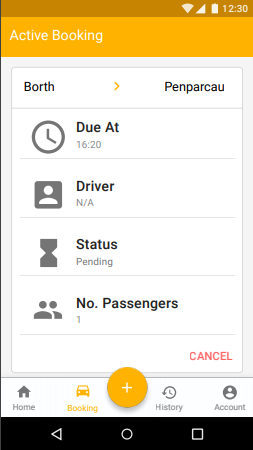
\includegraphics[width=\linewidth]{Resources/img/booking_overview_prototype.png}
		\caption{UI Prototype}
	\end{subfigure}
	\begin{subfigure}[b]{0.4\linewidth}
		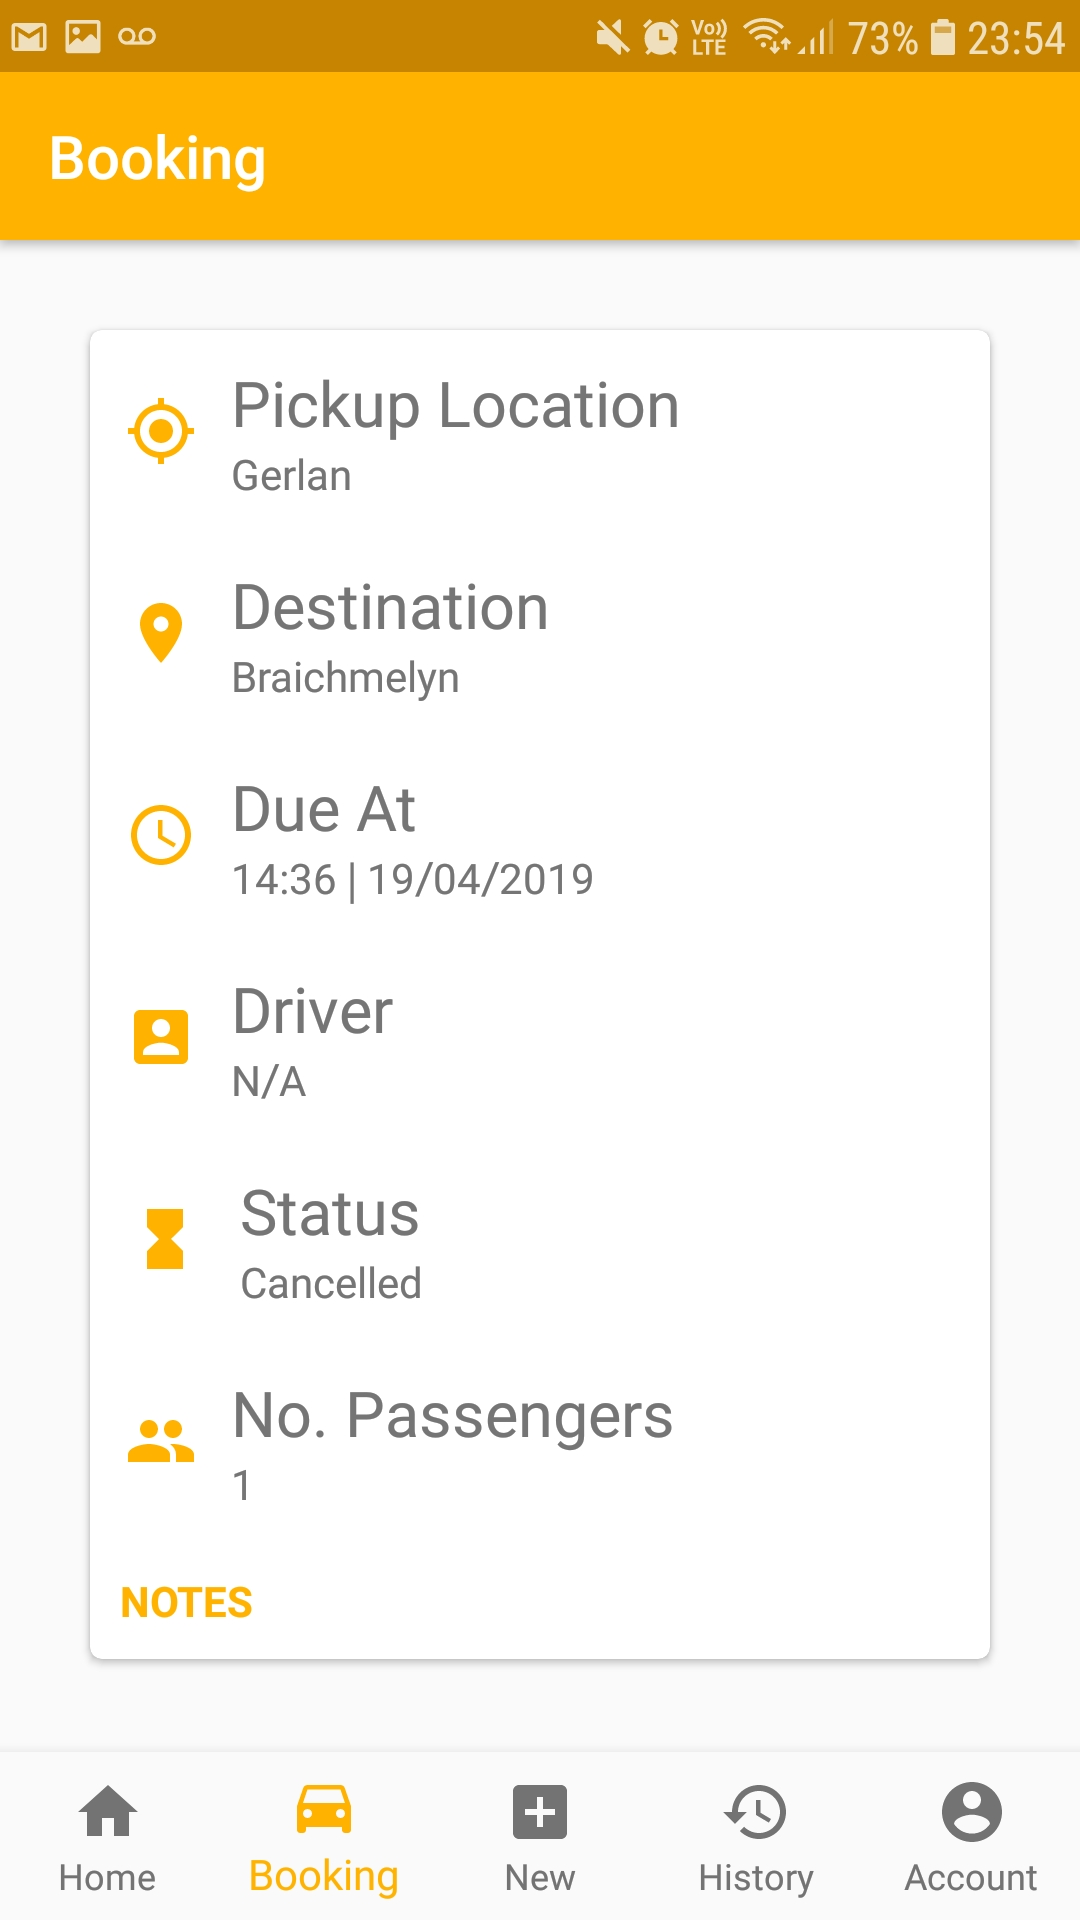
\includegraphics[width=\linewidth]{Resources/img/booking_overview_real.jpg}
		\caption{Actual Implementation}
	\end{subfigure}
	\caption{A comparison of the Booking Overview screen prototype and actual implementation}
	\label{fig:ui_compare}
\end{figure}

\newpage

\section{Week 2 (23/02 - 01/03)}
The focus of the second week of implementation was to get the REST API up and running and supporting all User related tasks: Registration, Authentication, and Account Management.

\subsection{Node.js Project Creation}
The very first step to implementing the API was to create the Node.js project and configure it to run in a Docker container alongside MongoDB. In order to create the Node.js project. An excellent GitHub repository~\cite{js_guidelines_documentation_ref} was discovered that outlined the best practices and standards in JavaScript projects.

\subsection{Containerization of Project}
Containerization of the API itself proved to be very straightforward, as it is a well-documented process and simply involved the creation of two files: Dockerfile and docker-compose.yml. The difficulty arose when attempting to connect the API container with MongoDB in order to persist data. The solution appeared to be to include a second container dedicated to MongoDB. This was working and a successful connection to the database could be made from within the API. However, in order to support data persistence after the containers were terminated, Data Volumes were required. A very helpful Medium tutorial~\cite{docker_medium_tutorial_ref} was used to correctly set up the data volumes and the setup was now working as intended.

\subsection{Authentication}
During the prototyping phase of development, an authentication API was created as a piece of spike work. Alongside this spike work, research into third-party authentication libraries was also done, with libraries such as Okta~\cite{okta_documentation_ref} and Passport.js~\cite{passport_documentation_ref} being considered. It was eventually decided, however, that a custom solution would allow for more fine-grain control over the API's authentication.

In order to provide the best security for the API, a token-based approach to authentication was used. It was also believed this would make the consumption of the API easier for the mobile application, by removing the need for sessions; thus making the API truly RESTful. The core principle behind this approach is that the user would send their email and password to a specific route within the API via Basic Authentication (Base64 encoding). The credentials would then be decoded and verified against the password hash stored in the database. If valid, the API would then provide the user with a 24-hour access token, to be sent in the header of any subsequent requests. Although initially requiring a bit of thought and research, implementation of this approach didn't provide any considerable difficulties. An excellent and in-depth tutorial written by Raj Amal~\cite{nodejs_authentication_tutorial_ref} was used as a reference to assist in the implementation.

\section{Week 3 (02/03 - 08/03)}
Testing of the API's current routes and consumption of the API by the Android App was the main focus of the third week.

\subsection{API Testing}
With the API already running inside a Docker container, the testing process was much more portable. Two testing libraries were used: Mochajs~\cite{mocha_documentation_ref} as the primary testing framework and Chaijs~\cite{chai_documentation_ref} as the assertation library. Whilst gaining familiarity with the testing libraries, Samuele Zaza's tutorial on Scotch.io~\cite{mocha_chai_tutorial_ref} was invaluable. The API was tested on a per-route basis, with several different cases for each route being tested. There was a bit of difficulty getting the tests to run seamlessly within the Docker container in TravisCI's environment. However, improved Docker Compose configuration eventually solve these issues, with assistance from Joe Cieslik's article in Hackernoon~\cite{docker_testing_tutorial_ref}.

\subsection{Implementation of Android App}
Consumption of the API by the Android App was where the bulk of the work took place during this week of development. Having already created a prototype App to consume an API using Retrofit and rxJava, much of the concepts and the boilerplate code was already in place. The difficulty came with refactoring the code to ensure reliability and good design practices. A major part of this was the implementation of the Model, View, ViewModel design pattern. An article on Medium.com by Ahmad Shubita~\cite{mvvm_tutorial_ref} was used to get to grips with the design pattern and its implementation via Retrofit.

Another essential aspect of the consumption of the API by the Android App was Error Handling, this is especially true for the registration process. In order to fully support internationalization/localization within the app, it was important that English error messages from the API not be displayed directly to the UI. Rather that error responses from the API come with four attributes: 'name' - the name given to a particular error; 'code' - an arbitrary number associated with a given error; 'message' - the error's name displayed in a more human-readable way; and 'description' - a brief description of the nature of the error. This way, the mobile app that consumes the API can simply read the code associated with a given error and fetch the matching string resource. One notable downside to this approach is that it increases the maintenance required. For example, if updates are made to the API that affects its error handling (a new error is added), this change must be accounted for in the App's Error-Parser.

\begin{figure}[!htb]
	\centering
	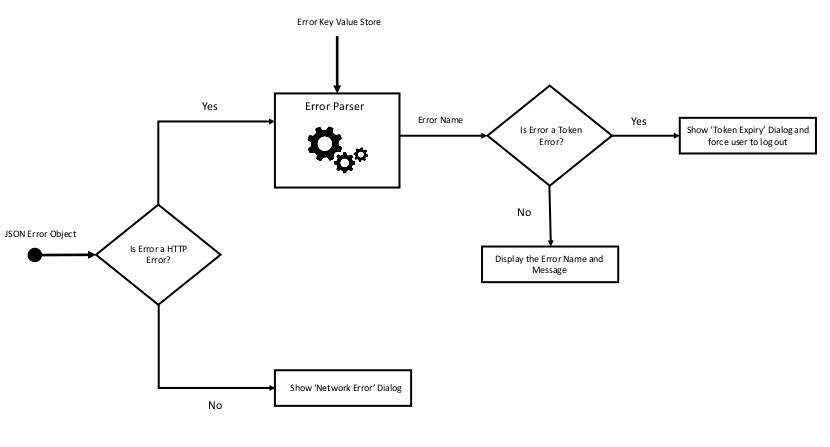
\includegraphics[width=\linewidth]{Resources/img/error_handling_flowchart.png}
	\caption{A flowchart depicting the error handling process within the Android App}
	\label{fig:error_flowchart}
\end{figure}

\section{Week 4 (09/03 - 15/03)}
The fourth week of development was mainly focused on preparations for the mid-project demonstration. Therefore, implementation of the platform itself was halted.

\subsection{App Deployment}
A major part of the preparations required for demonstrating the app's progress so far was the deployment of the API. Up to this point, the App had only been usable within an emulator ran on the same machine as the Node.js application. In order to properly demonstrate the app's development, it had to be able to access the API from an actual mobile device.

As discussed in Section~\ref{deployment}, it was decided that the API would be deployed on a local server box using the Node.js process manager and Nginx's reverse proxy. Although there are certainly benefits to using Docker in production, for example, reduced setup times and improved portability. Much of the research done heavily discouraged its use if inexperienced, especially in a self-hosted environment. Therefore, the decision was made to deploy the API without docker, however, it will continue to be utilized for development and testing environments.

The majority of the steps required to deploy the API were fairly straightforward and very well documented~\cite{deployment_tutorial_ref}. As discussed previously, there are certainly security implications associated with the chosen deployment approach. Such as lack of decent support for SSL, physical security concerns, inexperience with system administration, and the server itself being used for other, unrelated web applications. However, as a solution for demonstration purposes with fictitious personal data, it served its purpose excellently.

\section{Week 5 (16/03 - 22/03)}
With authentication already completed and supported both in the mobile app and on the REST API, the next logical step was to work on the implementation of booking creation. This task took surprisingly less time than anticipated, therefore there was time to complete some of the 'slack tasks'.

\subsection{Booking Data Model support whithin the API}
Having already implemented user authentication, creation, and management within the API, much of the foundations required for booking creation, management, and viewing were already in place. The main steps required were the following:

\begin{itemize}
	\item Create booking model
	\item Interact with booking model via service
	\item Create a controller to allow the router to interact with the service
	\item Implement all the necessary routes for bookings (CRUD)
	\item Add all the required input validations and error handling
	\item Write unit tests for each booking route
\end{itemize}

The booking model, service, controller, and router are all fairly standard and similar to those for the user data model. 

Input validation for booking creation was fairly trivial, with the exception of the 'time' field, as it had some special constraints:

\begin{itemize}
	\item Booking time cannot be further than 3 hours in the future
	\item Boking time cannot be sooner than 10 minutes away
	\item Booking time cannot be in the past
\end{itemize}

In order to easily compare time values, the ISO 8601 time stamp had to be parsed into a plain Javascript date object.

\subsection{Booking Creation support within the Android App}
Similarly to the API, having full support for the user data model within the App already made the implementation of booking creation very straightforward. Aspects of the App such as error handling and validation had to be updated to support the changes in the API.

The main challenge for this aspect of the implementation was the UI. A dedicated Activity was created for booking creation, with standard text inputs for pickup location, destination, and notes. The number of passengers and booking time fields each have a custom dialog that prompts the user for an input. The number of passengers dialog is a custom dialog that contains a number-picker, with the parent activity implementing its value listener. Therefore, whenever the value of the number picker is changed, the parent activity is kept updated. The time picker, however, is a default android time picker with the dialog all created programmatically. Therefore, tracking the selected value was trivial.

An interesting challenge faced when implementing the booking creation activity was deciding how to force the App to navigate to the 'booking viewing' screen upon successful creation of a booking. A considered option was simply to force the navigation whenever the booking creation activity was closed. However, this would prompt navigation even when the booking creation was canceled, which was an undesired behavior. The solution eventually implemented was to launch the booking creation activity with Android's 'startActivityForResult()' method. This would allow the activity to provide a return code when exited, meaning the activity could either exit with success or failure. If exited with success, a toast message is shown and the navigation is changed.

\subsection{Account Management within the Android App}
As mentioned at the start of this section, the primary tasks for this week's implementation took less time than anticipated. Therefore there was time to implement some of the less essential features. 

Given that the support for account management was already supported in the API, it made sense to create the UI for account management. The main features of the account screen are a circular avatar with the user's first name initial and a list of account actions. All of the account actions were implemented with the exception of changing password. This required further security precautions within the API.

\subsection{Support Dynamic Orientation within the Android App}
The next functionality to be addressed was landscape support, up until this point the app had been locked into portrait mode for simplicity. Most screens ported over to landscape fairly easily, given that the Constraint Layout was used for most screens and is typically well supported in both landscape and portrait modes. However, the account overview screen required its own layout file specifically for landscape mode. Luckily, Android makes this very easy with the use of the 'land' suffix in resource folder names. A new resource folder named 'layout-land' was created to contain the landscape specific layout. 

Allowing the app to be rotated did present some unexpected complications,  specifically concerning asynchronous API calls. When a fragment or activity is destroyed, any outstanding asynchronous subscriptions are terminated (to avoid dangling). This does, however, mean that whenever a view is destroyed and re-created due to orientation change, any outstanding API calls are discarded. A simple, yet arguably lazy solution to this issue was simply to lock the orientation in place whenever an API call is made, then to unlock the orientation upon completion.

\subsection{Welsh Language Support within the Android App}
Having gone to the effort to support internationalization/localization within the app, it made sense to add string values for another language. This was trivial and simply involved translating all the existing string values and adding them to a '-cy' resource directory.

\section{Week 6 (23/03 - 29/03)}
This week's development was almost entirely based on the Android App. It primarily involved full support for bookings via implementation of the following: Active Booking Overview, Booking Cancelation, Booking History. Password changing was also re-visited.

\subsection{Active Booking Overview}
The user's currently active booking could be retrieved by simply retrieving their most recent booking. This is guaranteed to be accurate as new bookings cannot be created whilst an active booking already exists. The booking overview screen simply contained a card view with information populated by the API request. The card view is populated using Android's Data Binding library, allowing for stricter conformity to the MVVM design pattern.  Unfortunately, the view does need to be manually refreshed to fetch up to date data. However, this is made intuitive through the use of Android's SwipeRefreshLayout. The view is also refreshed whenever the user changes navigation.

\subsection{Booking Cancelation}
After implementing the booking overview screen, adding support for booking cancelation was trivial. A text-button was added to the bottom of the card view. Pressing the button prompts a simple confirmation dialog to the user. If confirmed, a request is sent to the API to update the booking's status to 'Cancelled'.

\subsection{Booking History and Custom JSON De-Serialization}
As seen in Figure~\ref{fig:entity_relationship}, the way bookings are stored under a user's record in the database is as an array of MongoDB Object IDs. Therefore when a user is retrieved from the API, their bookings are shown simply as a list of Object references. Whereas the booking history list is required to display a limited amount of information about the booking. Although technically each booking could be retrieved fully by making a GET request to the API for that specific booking, this is an undesirable solution and would require significantly more API requests. Therefore a new route was implemented within the API specifically to retrieve a full list of a user's bookings. Mongoose's 'populate' function proved very useful for this purpose. 

The newly created route does not populate the 'driver' and 'customer' fields of the booking. Meaning they are still represented as strings (object IDs), whereas the booking model within the App stores the driver and customer fields as User objects. This caused some unexpected complications when it came to de-serialization of the JSON booking objects. When the booking JSON object was returned from a GET request to the /bookings/ route, it would be de-serialized just fine (due to driver and customer being populated). Whilst, if the booking JSON objects were returned from the /users/{id}/bookings route, a de-serialization exception was thrown. Upon further research, it was discovered that custom GSON de-serializers could be created that accounted for dynamic JSON fields. Although it took some time, this was done relatively easily and the problem was resolved.

The remainder of the implementation for booking history went off without a hitch, a boilerplate Recycler View Adapter was created to handle the list of bookings. With a click listener to open an Activity and display the booking's full details. The booking overview fragment created earlier in this section was re-used here.

\subsection{Password Changing}
All of the UI elements required for supporting password changing were already implemented. An update to the user updating route on the API was required in order to force the user to provide a valid previous password before the changes could be approved.

\section{Week 7 (30/03 - 05/04)}
This week's primary focus was adding support for the Driver role within the platform. There was also some time to implement the app's home screen and re-assess how notes were being handled within bookings.

\subsection{Supporting the Driver Role}
In order to fully support drivers within the API, a few changes needed to be made. The User model had to be updated to include fields for the driver's availability and company. This was fairly straightforward and simply required the addition of the fields to the model file and support for their update in the PATCH route. Some extra authorization checks were required for the user PATCH route, to ensure a user would only be able to change their own role under specific circumstances (resignation from a company).

All other aspects of the user model were already designed to accommodate users of different roles. For example, the 'bookings' field required no change as it could serve different purposes depending on the user's role. 

It was also predicted that certain routes in the future would need to be 'role-protected'. Therefore a very simple role-based access control middleware was created. The middleware could be applied to any route and either a single role or a list of roles could be authorized for that given route.

\subsection{Redesign of the Booking Notes System}
Having initially opted that a booking's notes be a single, optional string. It was decided that the support for communication this provided was very minimal. It's only purposed so far was to allow a Customer to make 'special requests' along with their booking. However, it was realized that a collection of notes within a booking that could be added by both the Customer and the Driver could potentially serve as a very simple communication mechanism. Notes would also be added by the system itself to inform users when changes to their booking have occurred, for example, status changes.

Implementing the new booking notes system on the API was very straightforward, it simply required a different type within the Booking model; together with support for appending notes to a Booking via its PATCH route.

\subsection{The App's Home Screen}
The last bit of development for this week of implementation was the fairly small task of implementing a home screen for the app. The layout and contents of this screen were decided a long time ago in the prototyping phase. Therefore the only required work was creating the screen's XML layout for both portrait and landscape orientations and implementing the API requests required. The information needed for the home screen required two requests be made to the API: one for the user's information (name, role, number of bookings) and another for the user's most recent booking information.

\section{Week 8 (06/04 - 12/04)}
This was the last week of development on the Android App, quite a lot of functionality was added. Primarily, complete support for Drivers within the App and updates to the booking overview to support the new notes system. In addition to developments within the App itself, it was also required that preparation work be done in the API, to support the Company Admin Web App.

\subsection{Supporting the new Notes System within the App}
In order to support the new notes system that was developed in the previous week,  a new Activity was created to serve as a 'notes view'. This new activity also contained a Floating Action Button that opened a text input for the user to append a new note to the booking. The only minor obstacle encountered in this implementation was that notes were simply an array of strings with no date stamp. Therefore in order to display them in semi-chronological order, the returned array was reversed (as they were being appended to the back of the array within the database).

\subsection{Implementing all the Driver Featuress within the App}
In order to implement all the functionality required for drivers within the app, surprisingly little work had to be done. The main tasks involved: The addition of an availability switch; an option to resign from their company; removal of 'booking creation'; support for viewing several active bookings; and support for updating a booking's status.

The addition of an availability switch and resignation option was fairly straightforward, the most difficult aspect was displaying an alternative 'home screen' and 'account overview' depending on the user's role. This was done by storing the user's role in the App's shared preferences and using this value to determine what version of each dynamic screen was loaded.

The API had already been updated to prevent drivers from creating bookings, however, the navigation option and booking creation screen were still very much available. It was decided that simply removing the 'new booking' option within the app's navigation for Drivers was the best solution. This was achieved with the addition of a second XML navigation menu, the required menu was then loaded into the Navigation Bar as needed. If the user opted to resign as a driver from within the App itself, the dynamic aspects of the app such as the Navigation Bar, Home Screen, and Account Screen were automatically changed to 'Customer Mode'. However, if the user was forcibly 'demoted' by their Company's Management, the App would not automatically update the required screen. 

Although still not ideal, the best conceivable solution was to query the user's role whenever a request is made to the API. This is when the most up-to-date information regarding the user is retrieved and the App could then select the correct 'mode' to display. However, unavoidably, the user's token would still contain a payload that indicated their role was 'Driver'. Therefore any attempt at the booking creation would be rejected. This problem would also persist if the order of role change was the other way around (Customer to Driver). It was ultimately decided that if the App detected any change in the user's role, it would consider the user's 'session' as expired and log them out.

The final step required in order to fully support Drivers within the app was implementing the ability to view multiple active bookings at once and edit their status. Whilst implementing the Customer aspects of the app it was assumed that only one active booking could exist at any given time. However, there was already support for 'booking lists' (due to the History screen). Therefore the approach was to re-use the Recycler View Adapter used by the Booking History list and implement a new view for each 'entry'. Upon clicking on an entry in the active booking list, the original Booking Overview fragment could also be re-used to display details about the booking. However, some amendments had to be made to the Booking Overview fragment for it to be usable by Drivers, namely: Replacing the 'Driver' field with 'Customer', and the addition of an 'edit' button by the booking's status. Of course, these changes would only be available to Drivers. The Booking Overview fragment would use the same approach as the other 'dynamic' screens within the app in order to display the correct content based on the user's role.

\subsection{Implementing the Company Model within the API}
In preparation for the development of the Web Application that is targeted towards Company Admins, the API had to be adapted to support Companies. Because most of the design for Company support had already been conceptualized, implementing the model for the Company was fairly straightforward. The same steps required for implementing Users and Bookings were taken, including the creation of a model, controller, and service file. With all the required /companies/ routes also implemented.

The bulk of the work took place in deciding how Companies would receive bookings from Customers. In the early stages of development, it was hoped that bookings would be delegated to companies automatically, by the system. However, for simplicity and to give full control to the companies themselves, a virtual 'booking market' approach was selected. This would include a list of all unallocated bookings that have been created by Customers. A Company Admin can then view this list and chose to 'claim' a booking. Once claimed, the booking would be removed from the list and would have all the object references required to 'belong' to that company. The same principle would apply for allowing companies to 'release' a booking, back into the 'booking market'. This would effectively undo all of the object references from the 'claiming' process.

The above mechanisms were implemented through the addition of three new routes: GET /bookings/, PATCH /bookings/{id}/release, PATCH /bookings/{id}/claim. The routes have all the necessary access protections to ensure only authorized users can perform the actions (for example, bookings can only be released by the company that owns it).

\section{Week 9 (13/04 - 19/04)}
The final week of development focused solely on the implementation of the Responsive Web App. In order to serve some of the created screens within the Web App, some minor updates to the API were also required.

\subsection{Web App Implementation}
Although the primary focus during the prototyping phase was on the API and the Android App itself. Some low-fidelity pen and paper UI prototypes were also created for the Web App. It was eventually decided, however, that the best choice for the Web App's User Interface was to use a template~\cite{angular_material_documentation_ref}. This shaved off a lot of implementation time (that was becoming scarce at this point of development) and also provided a professional, consistent look and feel. Having used a Material Design template, it also matched the style that was established throughout the development of the Mobile App.

Thankfully, most use-cases for the Web App required only boilerplate Angular code to make requests to the API and display the results on the screen. Some code from a tutorial by Jason Watmore~\cite{angular_tutorial_ref} was adapted to create the access control and authentication aspects of the app. Bootstrap tables were mostly used to display information. Authentication and Access Control mirrored what had been done on the mobile app, with the user's access token being stored in local storage and attached to any HTTP request headers. Error Handling was also very straightforward, with any errors simply being displayed to the user via a notification element. The only downside to this approach is that error messages were being shown directly from the HTTP response, making the Web App unfriendly for internationalization. This is an area that given an opportunity for further development, would certainly be addressed.

\begin{figure}[!htb]
	\centering
	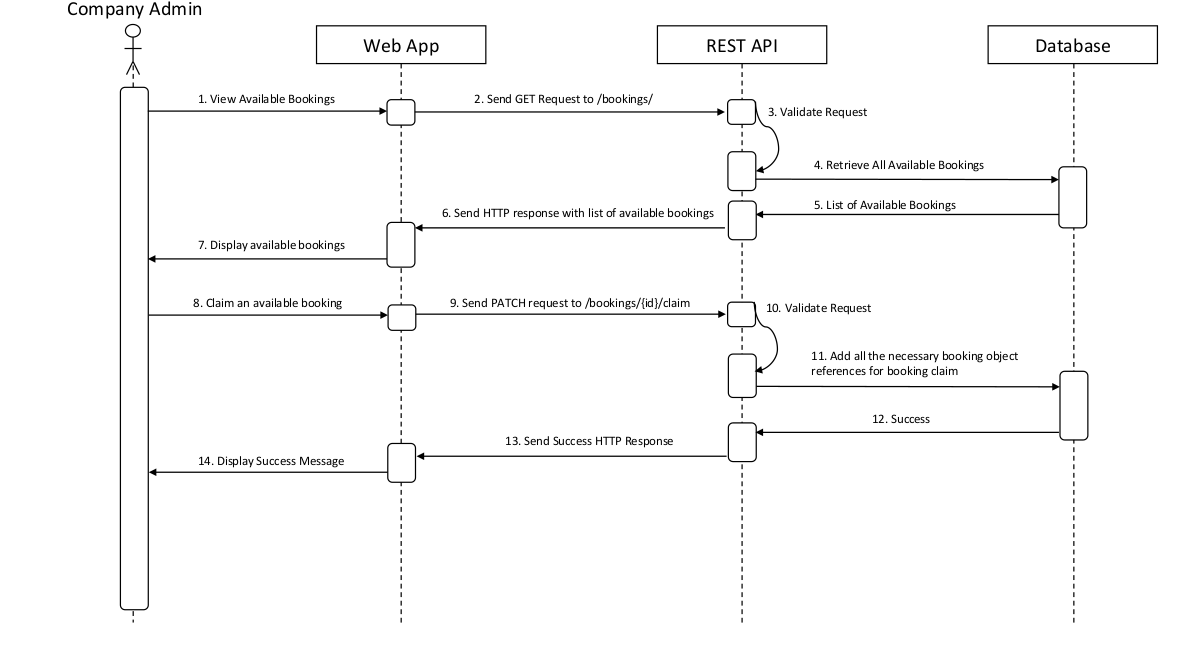
\includegraphics[width=\linewidth]{Resources/img/booking_claim_sequence.png}
	\caption{A UML Sequence Diagram showing the process of claiming a booking via the Web App}
	\label{fig:booking_claim_sequence}
\end{figure}

\subsection{Required Updates to the API}
Some aspects of the Web App's development called for changes to the API in order to be implemented successfully. The two most prominent examples are listing of a Company's Admins and recruiting drivers via their email. There was no dedicated mechanism within the API to retrieve a populated list of a Company's Admins, this was required for the Web App's 'company profile' screen. This addition was very simple and simply involved the creation of a new route 'GET /companies/{id}/admins' that retrieved a list of admins.

Another required change was supporting the addition of drivers to a company by their Email. Up to this point, Drivers had been added to a company by their Object IDs. However, this was not ideal, as Object IDs are long, complex strings that a user is unlikely to memorize or have access to. Therefore the 'PATCH /companies/drivers' route was adapted to support user emails as opposed to Object IDS.


\chapter{Testing}

\section{Outline of Testing Strategy}
The majority of the focus with regards to testing for this project was on the platform's REST API. This is arguably the most important system within the platform and is where most (if not all) security issues are likely to happen. Therefore it was important that each feature is tested thoroughly.

In addition to the rigorous testing of the API, manual testing was completed for the Android and Web App. Although there are very capable automated testing libraries available for both Android and Angular (JUnit, Espresso, e2e, etc). Primarily, due to short-term time constraints, it was decided that manual tests would be the best approach. The acceptance criteria of each requirement were used as the testing criteria for a given story. 

Some informal user tests of the platform were also done towards the end of development. The primary focus of these tests was to ensure everything was in order and functioning properly for the final demonstration. However, they served perfectly to compliment the testing strategy already in place. 

\section{Testing the API}
All of the API's testing was done on a 'per-route' basis, meaning, after successful implementation was completed, automated tests were written to rigorously test each route. This approach was selected because each of the platform's features was being implemented via a route within the REST API. Therefore it made sense to thoroughly test each route and by extension, each feature. There are roughly 5-6 tests for each route, making a total of 85 automated tests. 

\subsection{Testing Technologies Used}
In order to create the automated tests a few third party libraries were used: Mochajs, Chaijs, and Mockgoose. Mochajs was used to create a testing environment for NPM to run (within a Docker container). Chaijs is an assertion library with support for HTTP requests. Therefore within each test block, a Chai HTTP request was sent to the API and the response was evaluated using Chai's 'should' library.

Mockgoose is an NPM package that provides a test environment-friendly database by spinning up an in-memory MongoDB database. It 'catches' any requests made through Mongoose and forces them to be executed on the in-memory database as opposed to the standard data volume. By using an in-memory database tests can be run within the environment with zero consequence for the actual persisted data, whilst still maintaining the reliability of using a production DBMS.

\subsection{Regression Testing}
By using  TravisCI, the continuous integration tool all tests are automatically executed whenever the API is pushed to GitHub. If a test fails an email notification is sent out and the build is marked as 'failed'. This was invaluable during development to force regression tests to be executed whenever a new feature was pushed to the repository. Thus reducing the risk of bugs and hopefully increasing the correctness of the software.

\subsection{Stress Testing}
A major advantage of the chosen testing strategy is that automated tests can be used to accurately perform stress tests on the platform. For each route, a number of edge cases and fail conditions are tested. For example, for any route with input validation, attempted submission with invalid or incorrect input is simulated. The correct response to such a simulation is then asserted.

\subsection{Security Testing}
In addition to the stress testing undertaken, aspects of the API's security are also tested. For security testing, a mixture of automated tests and manual testing using Postman~\cite{postman_documentation_ref} were used. For example, most protected routes have automated tests to enforce the correct behaviour if invalid tokens are provided. The 'GET /users/{id}' route has an automated test to ensure that if a user's record is successfully retrieved their hashed password is not included in the response.

\section{Manually Testing the User-Facing Applications}
In order to test the user-facing applications within the platform as comprehensively as possible given the time restrictions, a manual approach was adopted. With acceptance criteria already being in place for each user story, the pass criteria of the manual tests were effectively already in place. 

Admittedly, much of the UI testing for the Android App was impromptu attempts at breaking or crashing the Android App. This was especially true with the Android App's handling of screen orientation. However, much of the UI testing also had a methodical approach. For example, when a new feature was fully implemented, a run-through of the process was done using Postman as the API's client. Then again using the Android App, then the results were compared to ensure correctness.

With regards to the Web Application's UI testing, many of the interface's elements were provided by reliable third-party code and were therefore inherently robust. However, some manual testing was done on the aspects of the interface implemented solely for the platform. The Web Application was also consistently tested for its support on various device resolutions.

\section{User Testing of the Platform}
As discussed at the beginning of the section, the platform in its entirety underwent informal user testing. Acquaintances had volunteered to simulate a potential use-case of the platform. One person would play the role of a customer using a mobile device, another would play the role of a driver, and a third would use a desktop device and play the role of a Company Admin. In order to fully commit to the simulation and hopefully give an idea of the platform's performance in a real-world scenario, the person playing the role of the driver used the Android App from a phone mount within a parked car.

The user testing was mainly focused on gauging the usability of the platform as a whole and preparing for the final demonstration. It was not intended to be a primary aspect of the testing strategy. However, having loaded the App onto one of the participant's devices (Samsung Galaxy S9 Running Android Pie), it was discovered that the App was throwing a network error. Because the App is consuming the API via HTTP, devices running a more up-to-date version of Android were rejecting the calls. The fix was simple and involved the simple addition of a line in the AndroidManifest file. However, if the test had not been completed, this issue would likely have occurred in the project's final demonstration.

\begin{figure}[!h]
	\centering
	\begin{subfigure}[b]{0.6\linewidth}
		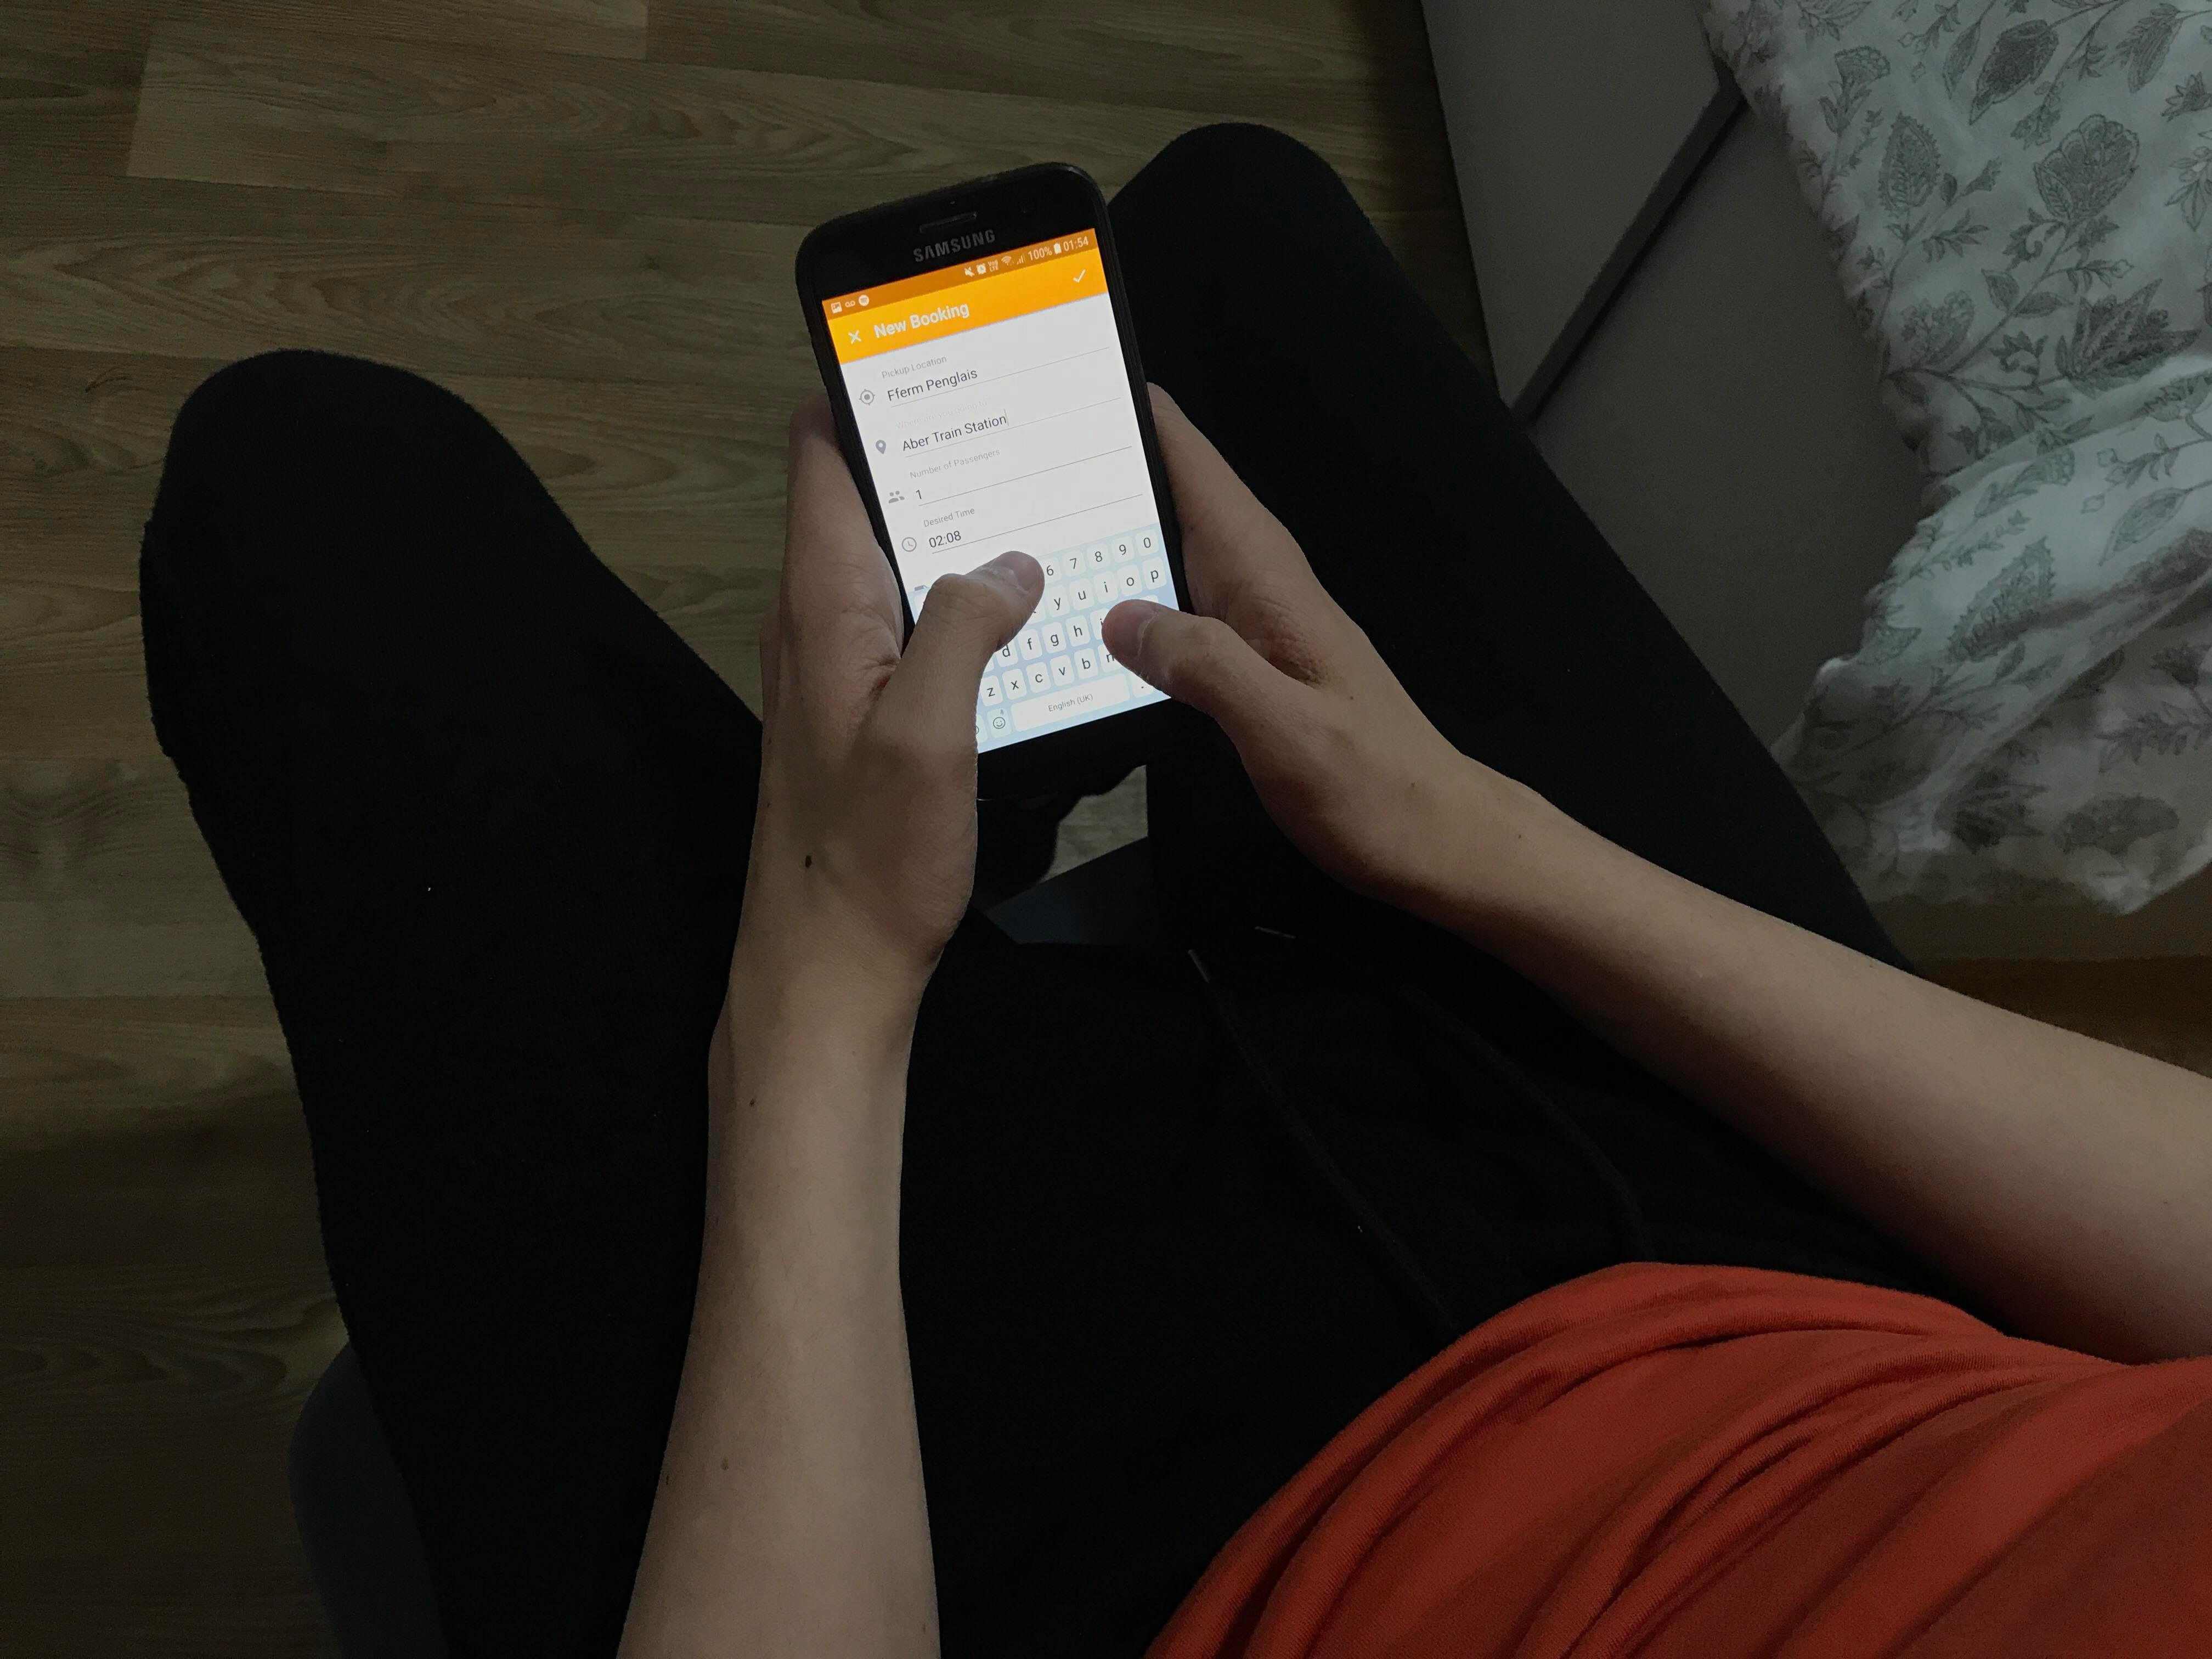
\includegraphics[width=\linewidth]{Resources/img/user_test_customer.jpg}
		\caption{Customer}
	\end{subfigure}
	\begin{subfigure}[b]{0.6\linewidth}
		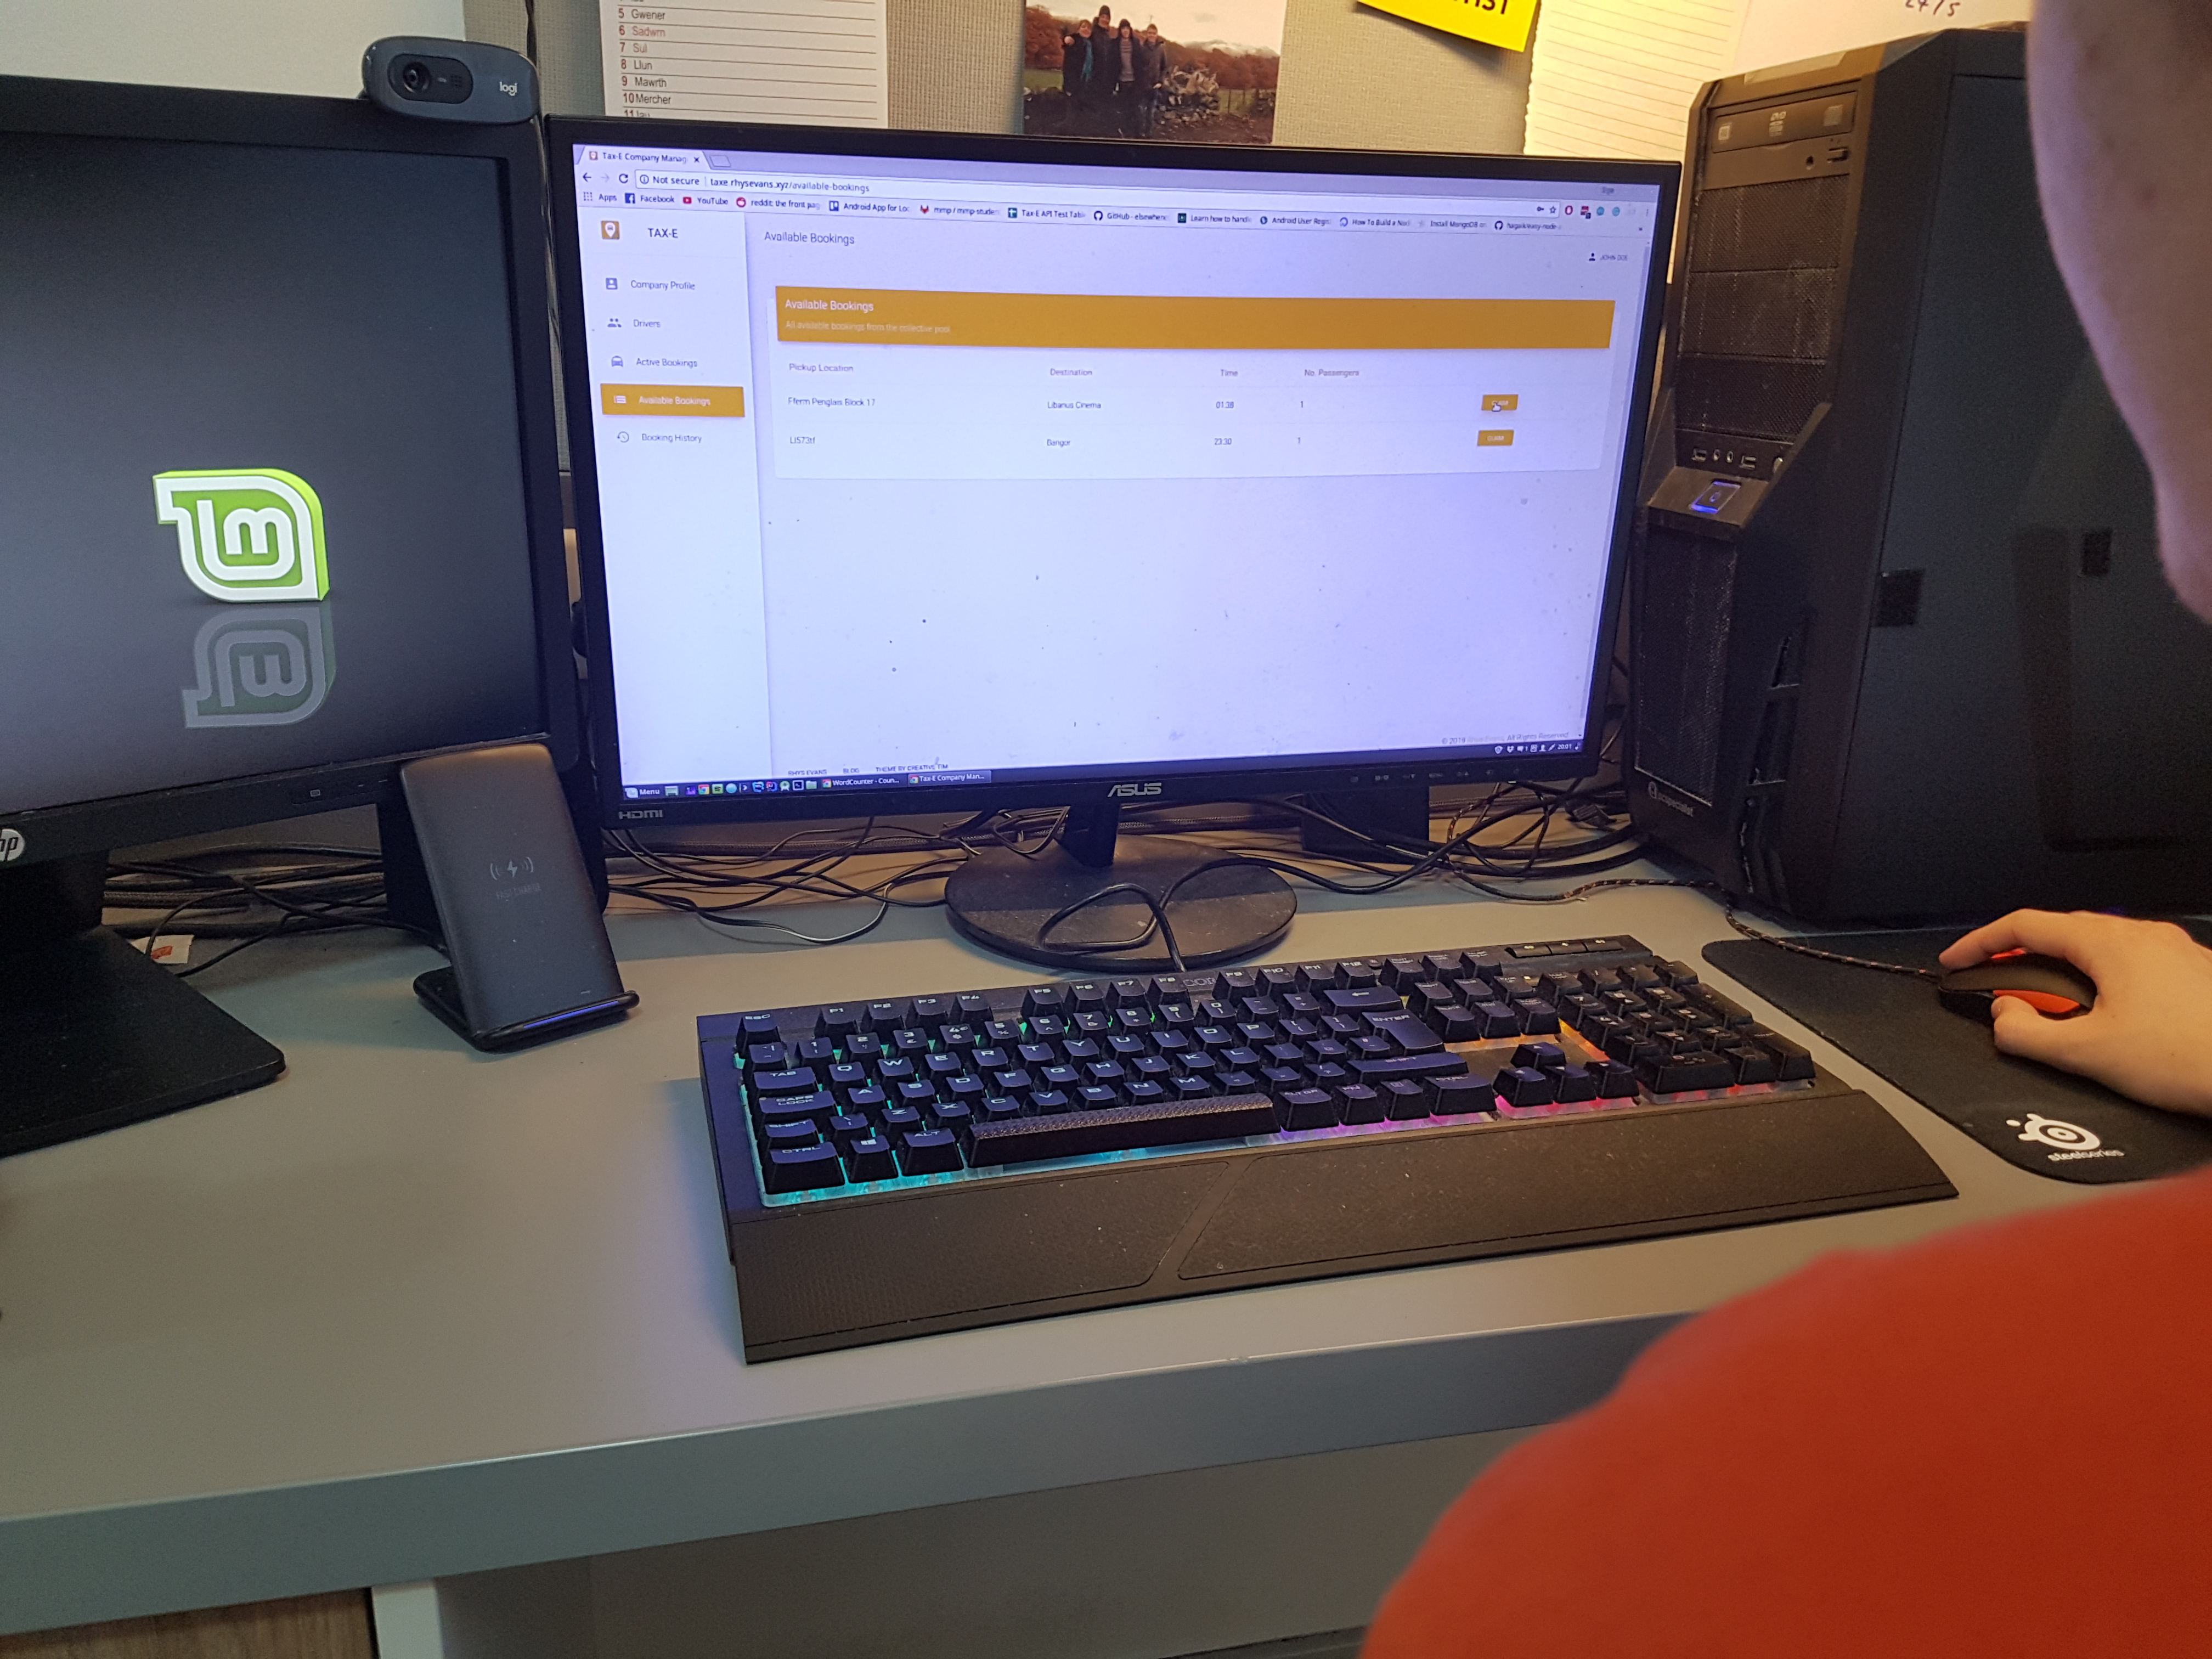
\includegraphics[width=\linewidth]{Resources/img/user_test_admin.jpg}
		\caption{Company Admin}
	\end{subfigure}
	\begin{subfigure}[b]{0.6\linewidth}
		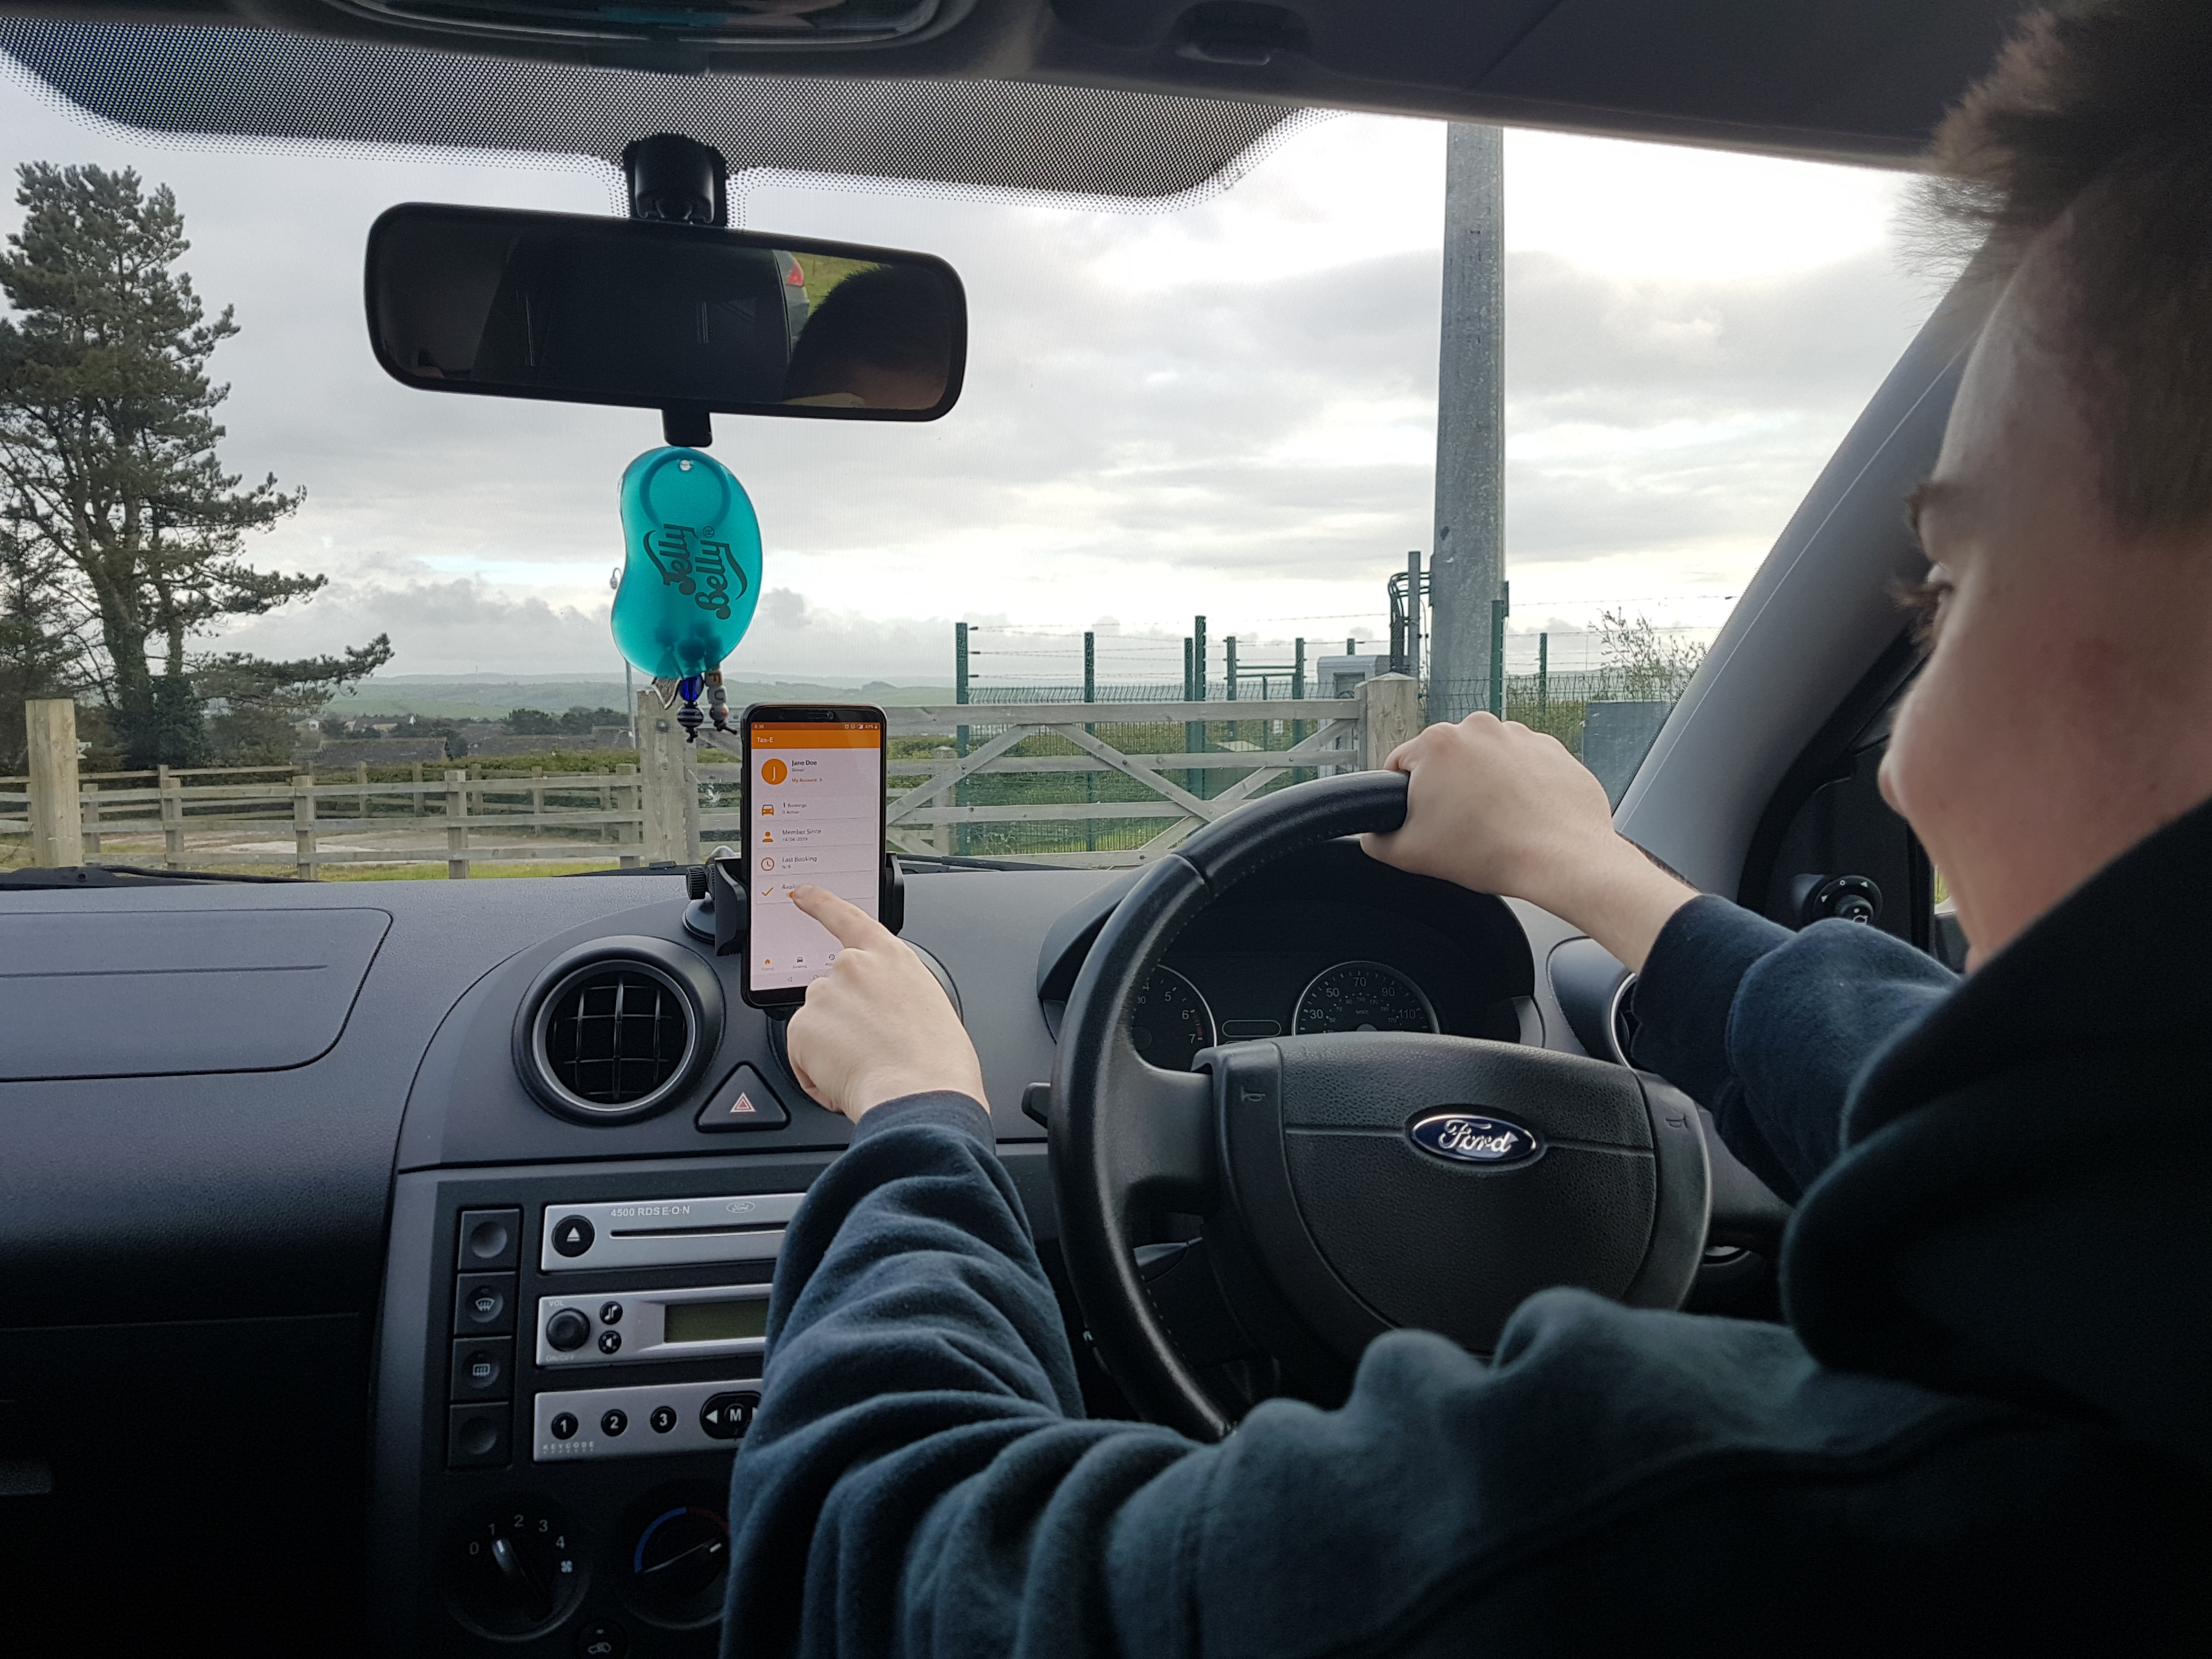
\includegraphics[width=\linewidth]{Resources/img/user_test_driver.jpg}
		\caption{Driver}
	\end{subfigure}
	\caption{Photographs of the User Testing Process}
	\label{fig:user_testing}
\end{figure}
\chapter{Evaluation}
As a whole, the project has been very successful, considering the aims set out at the beginning of the project and discussed in Section~\ref{ref_objectives}. The project has yielded a platform that is fit for purpose, developed to a relatively high standard and is objectively reliable. All of the proposed deliverables have been produced within the time frame provided.

However, as with any large project, especially where there is a limited amount of experience there are certain shortcomings and areas for improvement. This chapter will aim to critically evaluate every aspect of the project's production.

\section{Scope and Requirements of the Platform}

The 'requirements deliverable' was satisfied early in the development of the project. The requirements of the platform were arguably optimistic, however, they were completed nonetheless. A full set of User Stories was produced, which was stored and manipulated in several different ways during implementation as required by the development methodology used.

Identifying what was required from the platform was the most difficult aspect of this deliverable. Although there was a clear idea of what the platform's intended purpose and use-cases were. Extracting a clear and actionable set of requirements from this vision was easier said than done. This difficulty is likely the cause behind the slightly overly optimistic requirements. Another contributing factor was the lack of experience with large scale project management and the technologies used. Thus causing difficulty in estimation of tasks.

In future project management endeavors, more time would likely be allocated to the process of producing requirements. With more care and attention being given to the accurate estimation of tasks.

\section{Functionality}
The platform currently has all of the essential functionality implemented, with the exception of Mobile Notifications. Notifications were initially considered a key aspect of the platform and arguably, they still are. However, frustratingly, they were not implemented in the time frame of the project. This is solely down to time restrictions and poor estimation of the capability to complete the task within the time frame. In hindsight, perhaps the implementation of Notifications should have taken priority over a more non-essential feature. For example, the 'about' screen, or the name change support.

The spike work and plan for implementing Notifications was already in place. It was decided that Google's Firebase platform would be used to send push notifications to the mobile device. Whenever a user would log into the mobile app, their local device token would be sent along with the request and stored in their database record. Whenever a Notification needed to be sent to the user, the API would simply send HTTP request to the public Firebase API. The HTTP request would contain the message to be sent and the user's device ID.

\section{Deployment and Overall Security}
As has been emphasized several times throughout this report, the chosen deployment method of the platform was intended as a temporary solution for demonstration purposes only and is far from the ideal production environment. Node.js applications are conveniently portable, allowing a plethora of potential deployment options to be adopted with few implications for the REST API itself. However, the selected approach is a weakness nonetheless and the security implications should be discussed.

Given the chosen hosting platform for the Nginx reverse proxy (a home server running Ubuntu Server 16.04.3), support for SSL encryption via HTTPS was difficult to accomplish. In order to support HTTPS within the API, a self-signed certificate would have to be used, which would certainly have been more secure than plain HTTP. However, in order to support self-signed certificates in the API's clients, certificate validation had to be de-activated. Which was an (understandably) scarcely documented process, especially for Retrofit. Therefore, in order to spend more development time on the platform itself, it was decided that the deployment solution would only support HTTP.

In the context of security, if given more time for development, the following improvements would be considered:

\begin{itemize}
	\item Adoption of a commercial cloud hosting platform
	\item Rate limiting of API requests via Nginx
	\item Encrypted communications using SSL
	\item Only allow access to the API by approved clients (Android App and Web App) via unique service tokens.
\end{itemize}

\section{Potential Improvements to the Platform's Functionality}
Although the platform is currently fit for purpose and meets the objectives of the project. There are potential, mainly quality of life functionalities that could be added if the project was pursued further. Some examples include an automatic refresh of booking views when bookings are updated; GPS support for location selection and booking tracking; in-app messaging; profile views; automatic cancelation of a booking after a period of time has passed; automatic booking delegation.

Some of these features are elements of the platform that were initially considered to be within the scope of the project. For example, Figure~\ref{fig:location_picker} shows the UI Prototype for selecting the booking location via GPS.

\begin{figure}[!htb]
	\centering
	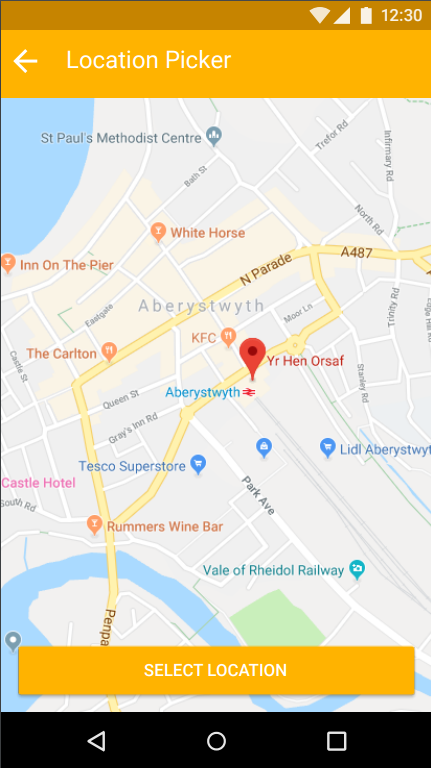
\includegraphics[width=0.5\linewidth]{Resources/img/location_picker_prototype.png}
	\caption{Prototype Screen for Picking Location via GPS}
	\label{fig:location_picker}
\end{figure}


\section{Conclusions}
This project was an invaluable learning experience. Both in terms of the technologies adopted and the project management aspects. The technologies and tools that were used worked together seamlessly. Given the modular nature of the platform, it is likely the case that any technology used for the API would integrate with the remainder of the platform with ease. The same is likely true for the choice of framework for the Web Application. However, having all the technologies be considered a common enough combination to have a designated acronym (MEAN stack) was certainly an encouraging sign.

The choice of Software Development Methodology was almost natural. The research into the correct way to implement an Extreme Programming approach paid off greatly. There was a bit of acclimatization required initially, and self-discipline to stick to the plan during each weekly cycle.
% add any additional chapters here

%TC:ignore
\setemptyheader

\nocite{*} % include everything from the bibliography, irrespective of whether it has been referenced.

% the following line is included so that the bibliography is also shown in the table of contents. There is the possibility that this is added to the previous page for the bibliography. To address this, a newline is added so that it appears on the first page for the bibliography. 
\addcontentsline{toc}{chapter}{Annotated Bibliography} % Adds References to contents page

%
% example of including an annotated bibliography. The current style is an author date one. If you want to change, comment out the line and uncomment the subsequent line. You should also modify the packages included at the top (see the notes earlier in the file) and then trash your aux files and re-run. 
%\bibliographystyle{StylesAndReferences/authordate2annot}
\bibliographystyle{StylesAndReferences/IEEEannotU}
\renewcommand{\bibname}{Annotated Bibliography} 

\bibliography{StylesAndReferences/references} % References file

\setemptyheader

\addcontentsline{toc}{chapter}{Appendices}
\chapter*{Appendices}

\pagebreak

% start the appendix - sets up different numbering
\fancypagestyle{plain}{%
%\fancyhf{} % clear all header and footer fields
\fancyhead[L]{Appendix\ \thechapter}
\fancyhead[R]{\leftmark}}

\appendix
\fancyhead[L]{Appendix\ \thechapter}
\fancyhead[R]{\leftmark}
\fancyhead[C]{}
\fancyfoot[C]{\thepage}
\renewcommand{\headrulewidth}{0.4pt}
\renewcommand{\chaptermark}[1]{\markboth{#1}{}}

\fancyhead[L]{Appendix\ \thechapter}
\fancyhead[R]{\leftmark}
\fancyfoot[C]{{\thepage} of \pageref{LastPage}}

% include any appendices here
\chapter{Third-Party Code and Libraries}
Bcrypt Js is a Javascript library to implement the bcrypt password hashing function. Version 2.3.0 is used within the platform to hash user passwords. The library is open source and available from the NPM website or GitHub directly: \url{https://www.npmjs.com/package/bcryptjs}. It is licensed under the MIT License~\cite{mit_license_ref} and is used without modification.

Basic-Auth is a Javascript library to parse basic authentication headers within Node.js. It is used within the platform to decode credentials using Base64. The version used was 2.0.1, the library is available from NPM directly: \url{https://www.npmjs.com/package/basic-auth}. It is licensed under the MIT License~\cite{mit_license_ref} and is used without modification.

Express is a minimalist web framework for Node.js. It was used within the platform in conjunction with Node.js to create the REST API. Version 4.16.4 was used. It is available from the NPM website: \url{https://www.npmjs.com/package/express}. It is licensed under the MIT License~\cite{mit_license_ref} and is used without modification.

JsonWebToken (jwt)  is an implementation of JSON Web Tokens for Javascript. It is used within the platform to generate access tokens with a payload for users. It is available via the NPM website: \url{https://www.npmjs.com/package/jsonwebtoken}. Version 7.1.9 was used. It is licensed under the MIT License~\cite{mit_license_ref} and is used without modification.

Mongoose is an Object Modelling Tool for MongoDB, it is designed to operate in asynchronous environments. Version 4.6.0 of this library was used within the platform to interact with the MongoDB database from the API. The library is available from the NPM website: \url{https://www.npmjs.com/package/mongoose}. It is licensed under the MIT License~\cite{mit_license_ref} and is used without modification.

Mockgoose is a Javascript library that allows MongoDB databases to be created in-memory for testing purposes. Version 8.0.1 is used within the platform's test suite to mock the backend database. It is available via the NPM website: \url{https://www.npmjs.com/package/mockgoose}. The library is licensed under the MIT License~\cite{mit_license_ref} and is used without modification.

Mocha is a Javascript testing library that provides an environment for tests to be executed in. Version 6.0.2 is used in the platform for testing. It is available on NPM: \url{https://www.npmjs.com/package/mocha}. The library is licensed under the MIT License~\cite{mit_license_ref} and is used without modification.

Chai is an assertion library intended to be used together with a testing library. Version 4.2.0 is used within the API for testing assertions and HTTP requests. It is available on NPM: \url{https://www.npmjs.com/package/chai}. The library is licensed under the MIT License~\cite{mit_license_ref} and is used without modification.

Retrofit is a Java library to convert HTTP requests into Java interfaces. Version 2.1.0 was used within the Android App to send HTTP requests to the REST API. It is available on GitHub: \url{https://square.github.io/retrofit/} and is licensed under the Apache License~\cite{apache_license_ref}. It is used without modification.

rxJava is a Java library by ReactiveX for creating asynchronous programs using observable sequences in Java. It was used within the Android App to create lifecycle aware, asynchronous HTTP requests. Version 2.1.0 was used and is available from GitHub: \url{https://github.com/ReactiveX/RxJava}. It is licensed under the Apache License~\cite{apache_license_ref} and is used without modification.

Material Dashboard Angular is a boilerplate theme for Angular, it provides both the angular code and the Bootstrap and SCSS required. For the purposes of the project, only the Bootstrap and SCSS aspects were utilized. With the Angular components used for reference. The free version was used and is licensed under the MIT License~\cite{mit_license_ref}. It is available on Creative Tim's website: \url{https://www.creative-tim.com/product/material-dashboard-angular2}, it was used with minor modifications to some colour variables.
\chapter{Ethics Submission}
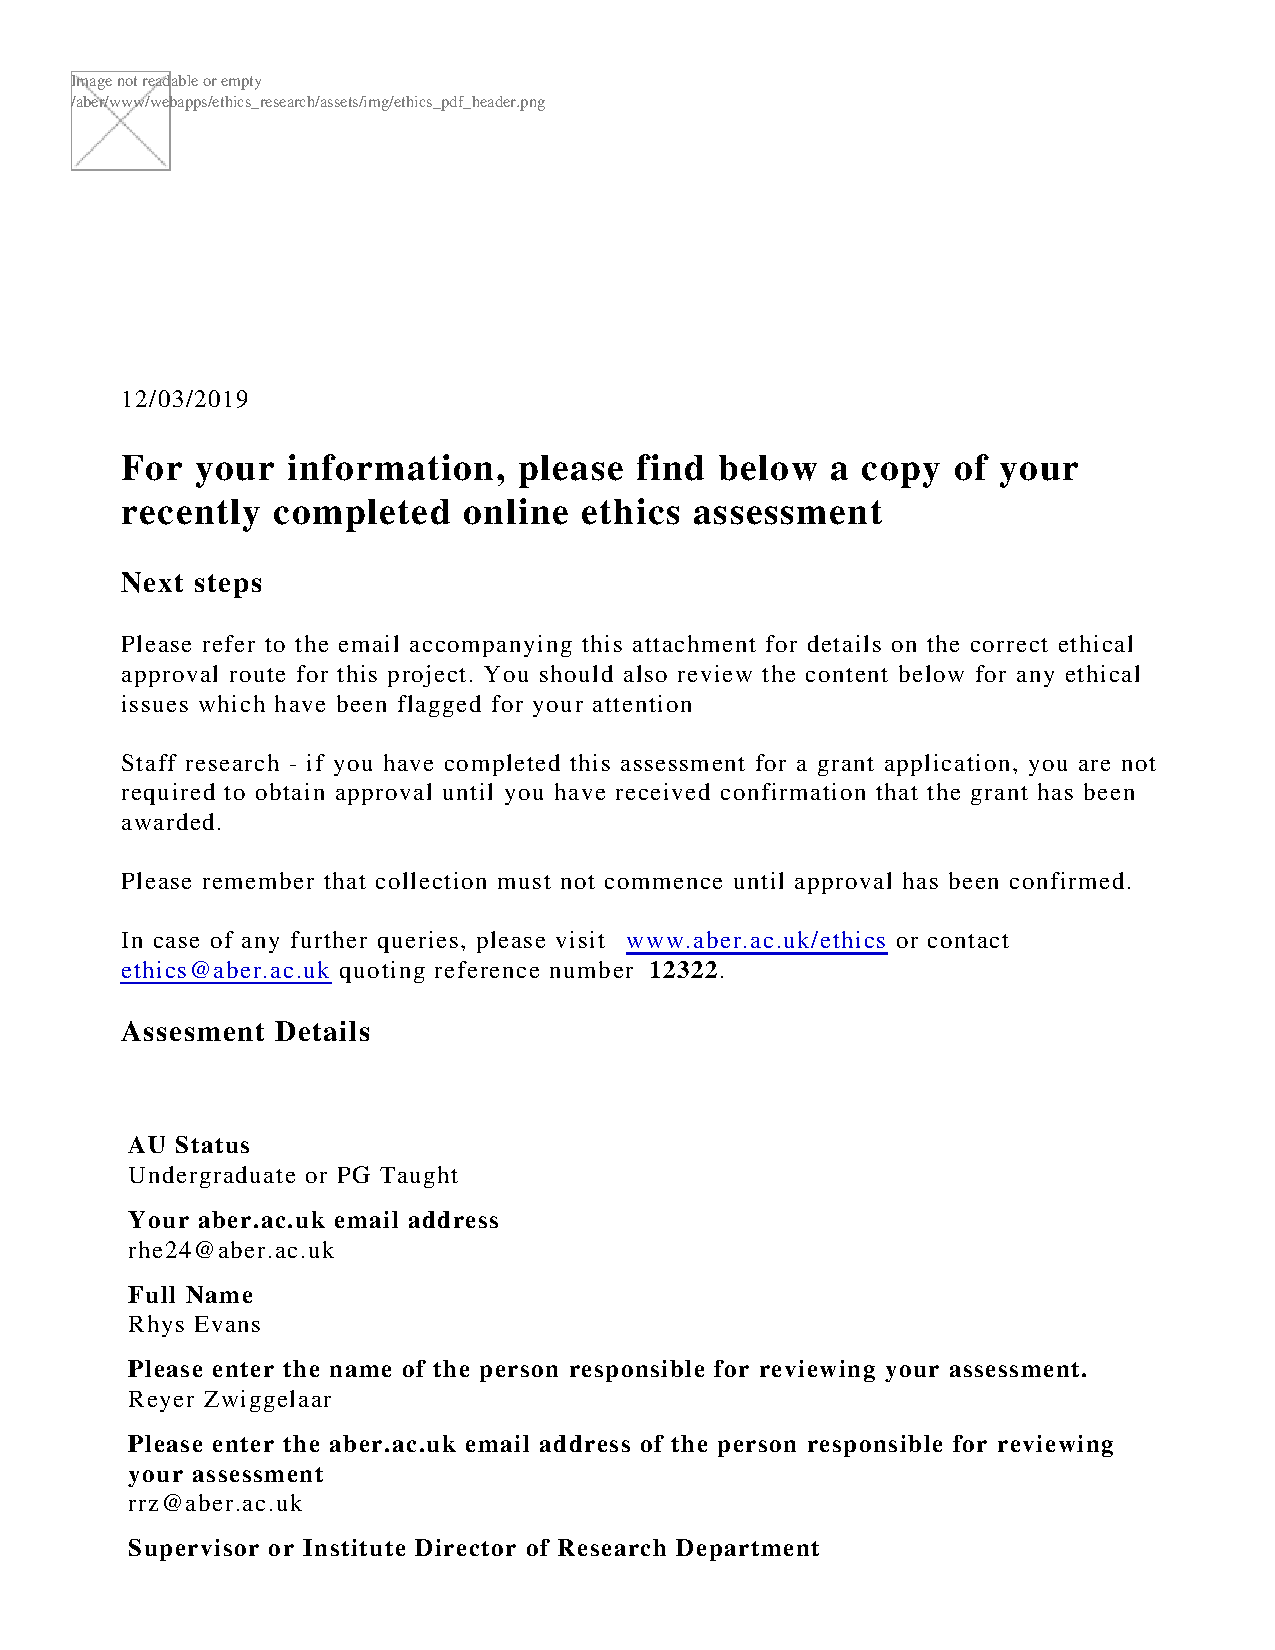
\includepdf[pages=-]{Resources/ethics_form.pdf}
\chapter{API Documentation}
During development of the API, a Markdown file was produced to serve as documentation for the API's routes, errors, etc. The documentation file was very useful when writing the HTTP requests from the client.

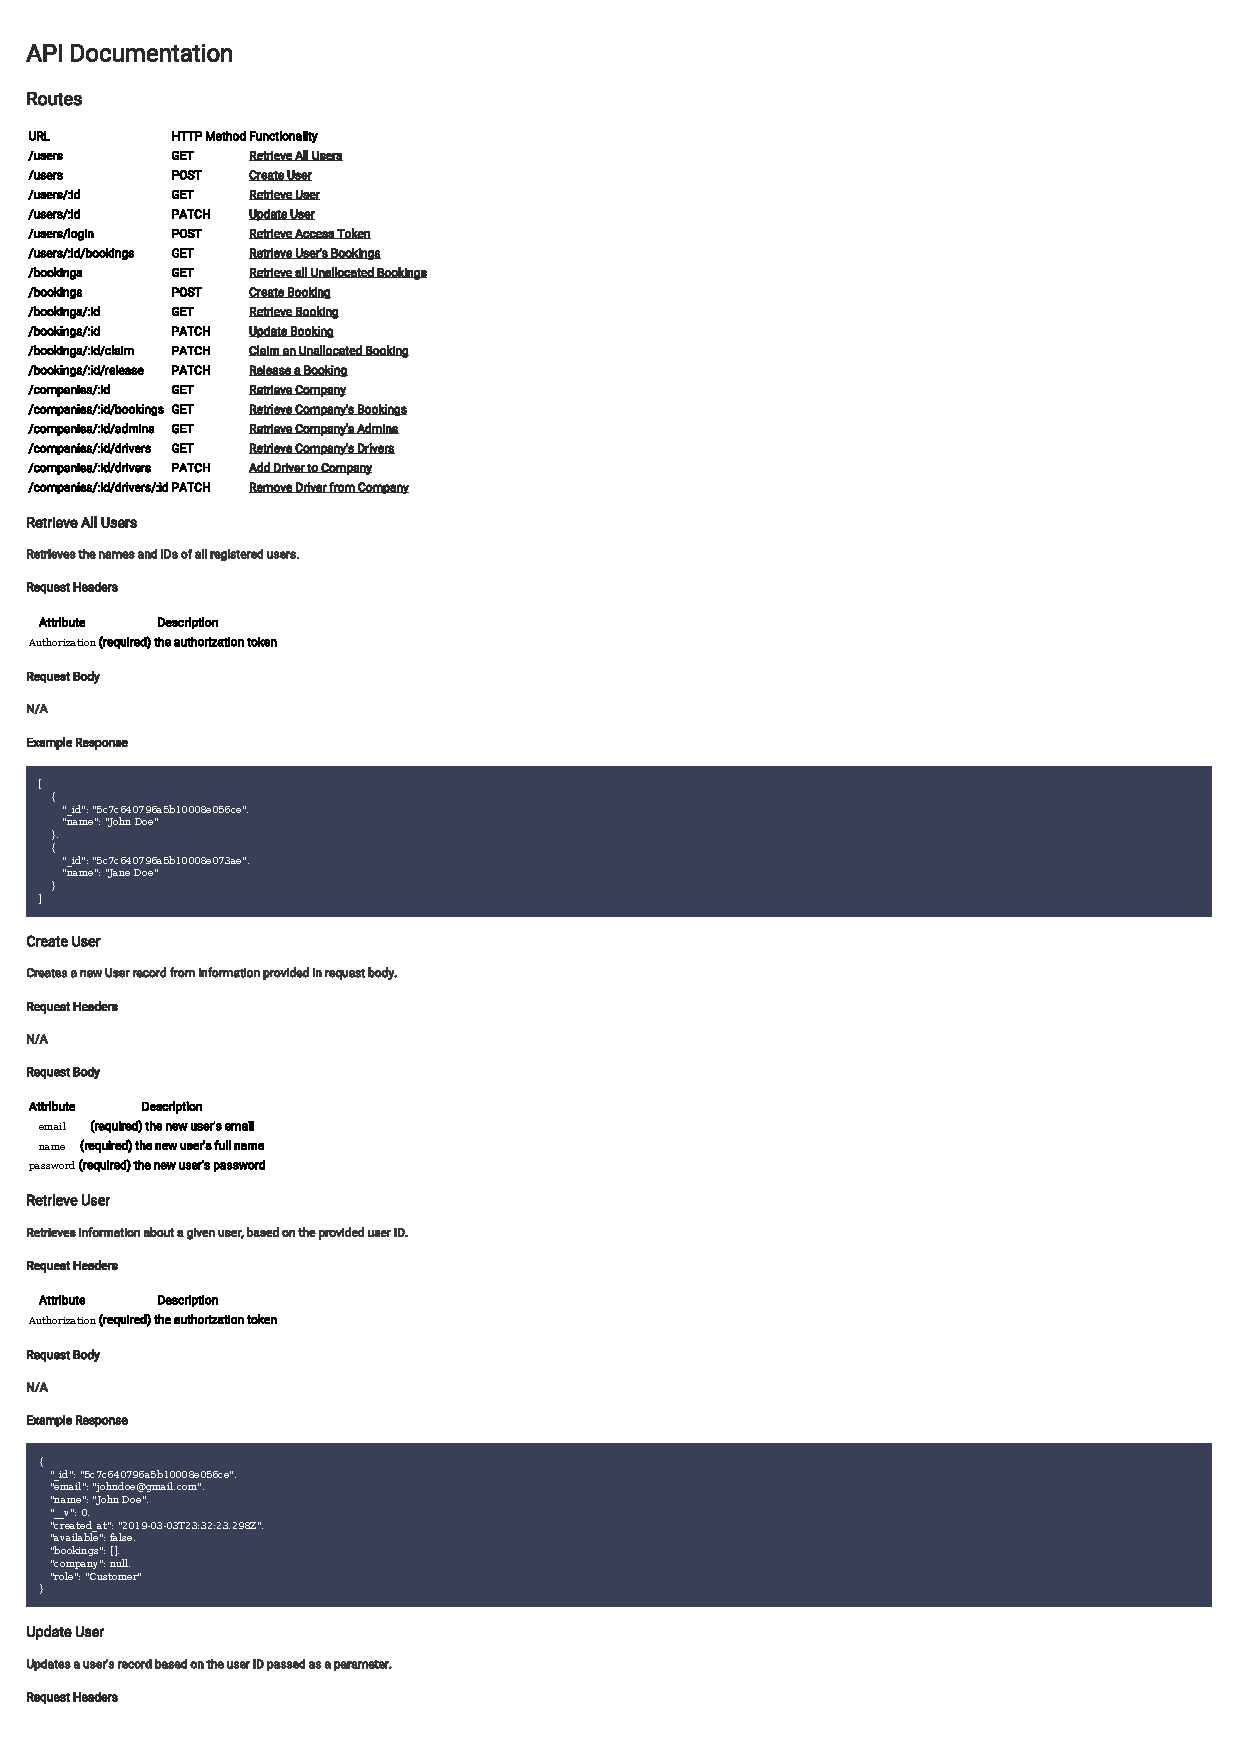
\includepdf[pages=-]{Resources/api_docs.pdf}
\chapter{User Stories Document}
After the creation of all the user stories, they were placed in a central document. This was so they could easily be copied over to any physical or electronic 'to do' boards, to ensure consistency.

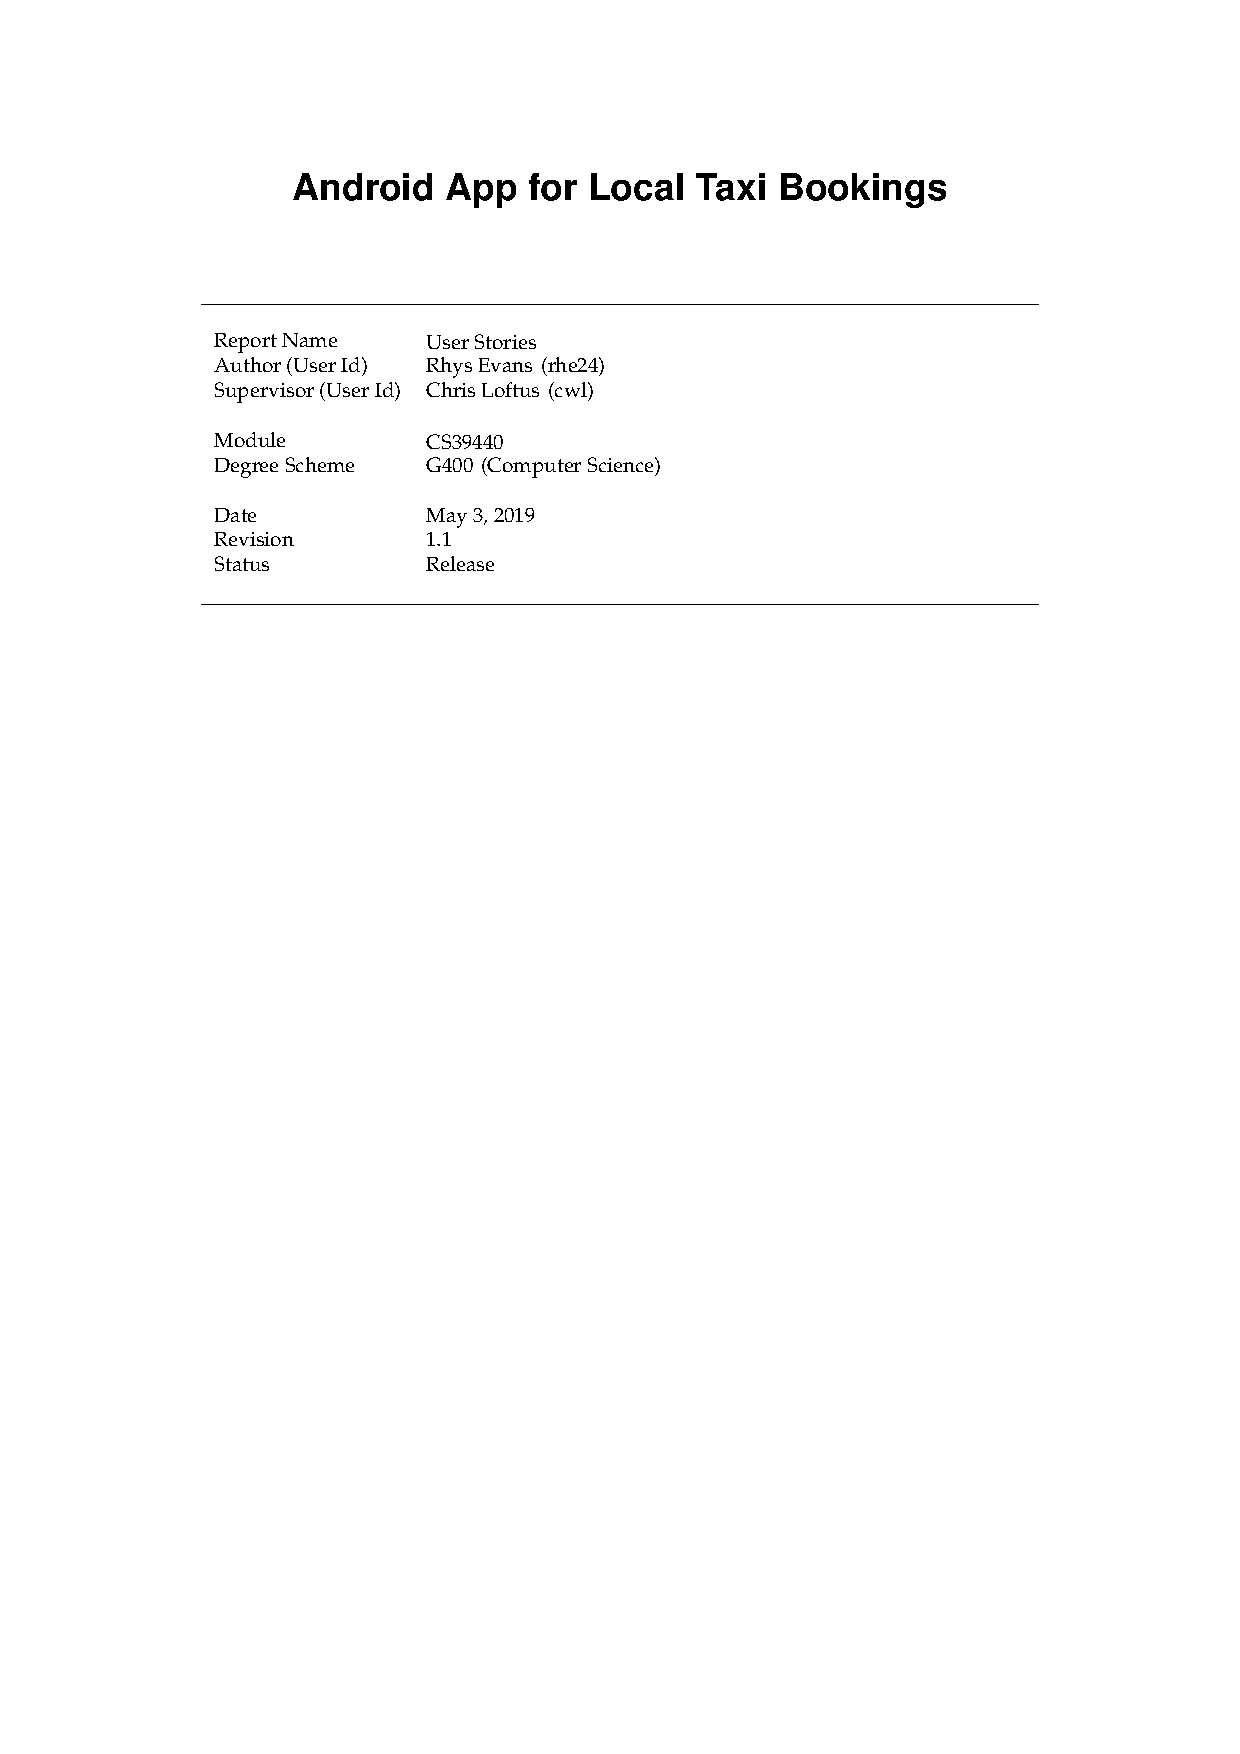
\includepdf[pages=-]{Resources/user_stories.pdf}
\chapter{User Interface Prototypes}
In the first week of development, several high-fidelity User Interface prototypes were created for the Android Application. In total there were 58 screens in order to showcase every functionality and some error and success cases. For purposes of keeping things concise, the entire document won't be included in this Appendix, only the 'essential' screens. The full document is available at: \url{http://blog.rhysevans.xyz/content/MMP_UIPrototypes.pdf}.

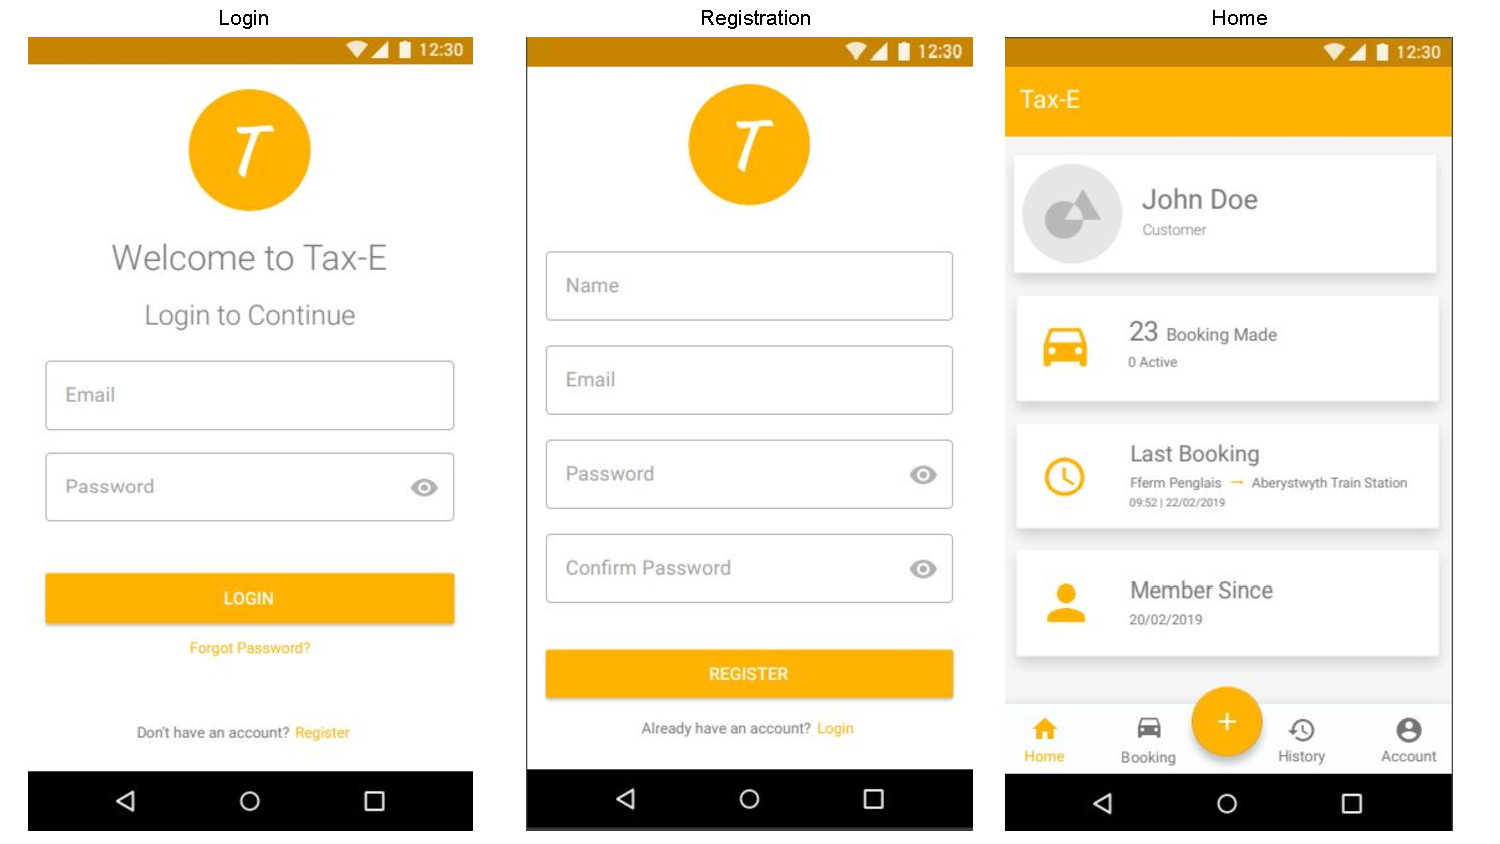
\includepdf[pages=-]{Resources/ui_prototypes.pdf}



\fancypagestyle{plain}{%
   \fancyhead{} %[C]{Annotated Bibliography}
   \fancyfoot[C]{{\thepage} of \pageref{LastPage}} % except the center
   \renewcommand{\headrulewidth}{0pt}
   \renewcommand{\footrulewidth}{0pt}
}

%TC:endignore

\end{document}
